\documentclass[a4paper, twoside, 11pt]{report}
\usepackage{derivation-nops}
\usepackage{main}

\title{Building Derivations}
\author{Justin Keung}

\begin{document}
\begin{titlepage}

\newcommand{\HRule}{\rule{\linewidth}{0.5mm}} % Defines a new command for the horizontal lines, change thickness here

%----------------------------------------------------------------------------------------
%	LOGO SECTION
%----------------------------------------------------------------------------------------


\includegraphics[width=6cm]{title/logo.eps}\\[3cm] % Include a department/university logo - this will require the graphicx package
 
%----------------------------------------------------------------------------------------

\center % Center everything on the page

%----------------------------------------------------------------------------------------
%	HEADING SECTIONS
%----------------------------------------------------------------------------------------

\textsc{\LARGE BEng Individual Project}\\[1.5cm] % Name of your university/college
\textsc{\Large Imperial College London}\\[0.5cm] % Major heading such as course name
\textsc{\large Department of Computing}\\[0.5cm] % Minor heading such as course title

%----------------------------------------------------------------------------------------
%	TITLE SECTION
%----------------------------------------------------------------------------------------
\makeatletter
% \vskip 5cm
% {\huge \@title}
% \vskip 1cm
\rule{\textwidth}{1pt} \\[0.4cm]
% { \huge \bfseries \@title}\\[0.4cm] % Title of your document
{ \huge \bfseries \@title} \\[0.1cm]
\rule{\textwidth}{1pt} \\[1.5cm]
 
%----------------------------------------------------------------------------------------
%	AUTHOR SECTION
%----------------------------------------------------------------------------------------

\begin{minipage}{0.4\textwidth}
\begin{flushleft} \large
\emph{Author:}\\
\@author % Your name
\end{flushleft}
\end{minipage}
~
\begin{minipage}{0.4\textwidth}
\begin{flushright} \large
\emph{Supervisor:} \\
Prof. Steffen van Bakel \\[1.2em] % Supervisor's Name
\emph{Second Marker:} \\
(Not published at the time of submission) % second marker's name
\end{flushright}
\end{minipage}\\[2cm]
\makeatother

% If you don't want a supervisor, uncomment the two lines below and remove the section above
% \Large \emph{Author:}\\
% Justin Keung\\[3cm] % Your name

%----------------------------------------------------------------------------------------
%	DATE SECTION
%----------------------------------------------------------------------------------------

{\large \today}\\[2cm] % Date, change the \today to a set date if you want to be precise

\vfill % Fill the rest of the page with whitespace

\end{titlepage}

\begin{abstract}
Proof assistants are tools that help users create and verify formal proofs. They have been used to help write reliable software, verify security protocols, and prove mathematical theorems.

More recently, people have created proof assistants to teach logic. They are designed to be more intuitive for beginners than industrial-grade proof assistants, at the cost of expressive power and proving ability. However, these educational proof assistants  support their own syntax and cannot let users easily modify the proof system in which the derivations are built.

This project presents \projectname{}, a web-based proof assistant which addresses both issues. It supports \LaTeX{} syntax and lets users modify the proof system through its web interface on the fly. Users can build derivation trees and arbitrarily modify the syntax and inference rules of the proof system. \projectname{} verifies the given derivation based on the proof system defined by the user.

\end{abstract}

\renewcommand{\abstractname}{Acknowledgements}
\begin{abstract}
I would like to thank my supervisor, Steffen van Bakel, for his support and invaluable feedback throughout this project. I seem to have come out of every meeting thinking a little sharper.

I would also like to thank David Davies for his feedback on this report, as well as my friends Aboud, Hamish, and Jerome for helping me test the web application.

Finally, I would like to thank my friends and family for their support.
\end{abstract}

\pagestyle{toc}
\pagenumbering{roman}
\tableofcontents
\listoffigures
% \listoftables
% \cleardoublepage

\pagestyle{fancy}
\clearpage
\pagenumbering{arabic}
\chapter{Introduction}
Proof assistants, or interactive theorem provers, are tools that help users create and verify formal proofs. Proof assistants like Rocq (formerly Coq) \cite{rocq}, Agda \cite{agda}, and Isabelle \cite{isabelle} have both practical and theoretical applications. Rocq is used to develop and formally verify CompCert \cite{leroy:2009}, a compiler for a large subset of the C programming language and intended for programming reliable embedded systems. In 2005, Georges Gonthier \cite{gonthier:2005} used Rocq to formalise a proof of the four colour theorem, which further clarified doubts about the original computer-assisted proof by Appel and Hakel in 1976 \cite{appel:1976}. Isabelle is used to formally verify the correctness of Transport Layer Security (TLS) \cite{paulson:1999}, a network security protocol.

More recently, proof assistants like Pandora \cite{pandora:2007, pandora}, Carnap \cite{carnap, carnap:2018}, Holbert \cite{oconnor:2022}, and Logitext \cite{yang:2022} have been designed to help students learn logic. They prioritise ease of use over advanced features and help students learn by providing instant feedback on their proofs. Students at Imperial who used Pandora, a proof assistant for Fitch-style \cite{fitch:1952} Natural Deduction, were found to approach exam problems more methodically, were less likely to make arbitrary assumptions, and were more precise in their proofs \cite{pandora:2007}.

However, these educational proof assistants share two key issues:
\begin{itemize}
    \item Each proof assistant supports its own syntax. For example, the universal quantifier ($\forall$) is represented by ``\lstinline{A}'' in Carnap, ``\lstinline{all}'' in Holbert, and ``\lstinline{forall}'' in Logitext. Before students can use the proof assistants, they need to learn unfamiliar syntax which not only does not apply to other proof assistants, but also does not match how they build derivations with pen and paper. This takes away time that could have been spent on learning the proof systems instead.
    \item None of the proof assistants investigated in this report lets users modify proof systems arbitrarily in a user-friendly manner. Among them, Carnap supports the widest range of proof systems, including Natural Deduction for first-order logic \cite{carnap:systems}, the Sequent Calculus \cite{carnap:systems}, and possibly the simply typed $\lambda$-calculus\footnote{The $\lambda$-calculus is not a pre-defined proof system in Carnap. However, Carnap-Core (the libraries which allow users to specify proof systems) supports proof systems with abstractions and applications \cite{carnap:2018}, so it should be able to support the simply typed $\lambda$-calculus.}. However, defining a new proof system, or modifying an old one, requires the user to work with the core libraries in Haskell and cannot be done on the fly.
\end{itemize}

This project presents \projectname{}\footnote{Embla is the first human woman in Norse mythology, mirroring the fact that Pandora is the first human woman in Greek mythology.}, a web-based educational proof assistant that addresses both issues:
\begin{itemize}
    \item Users can build derivations entirely using \LaTeX{} syntax. This means \projectname{} also uses its own syntax, since none of the educational proof assistants above support \LaTeX{}. However, students who already know \LaTeX{} will not need to spend extra time learning unfamiliar syntax, while students who do not know \LaTeX{} will be learning syntax that is useful outside \projectname{}, such as writing assignments and reports.
    \item Users can modify proof systems on the fly without any understanding of the implementation details of syntax and inference rules. Users only need to modify plain text input in the web interface of \projectname{}.
\end{itemize}

\section{Contributions}
The contribution of this project is \projectname{}, a web application with the following features:
\begin{itemize}
    \item Users can define syntax rules (\Cref{section:syntax}) and inference rules (\Cref{section:inference}). \projectname{} supports \LaTeX{} syntax and several shorthand notations. \Cref{fig:introduction:editor} shows what the user sees when editing the syntax and inference rules in \projectname{}.
    \item Users can build derivations in \projectname{}. It verifies whether the derivation is correct according to the syntax and inference rules defined by the user (\Cref{chapter:checking}). Prior to verification, both the inference rules (\Cref{section:inference}) and the derivation given by the user (\Cref{section:term}) are transformed into intermediate internal representations. \Cref{fig:introduction:builder} shows what the user sees when building a derivation in \projectname{}.
\end{itemize}

\begin{figure}[!htbp]
    \centering
    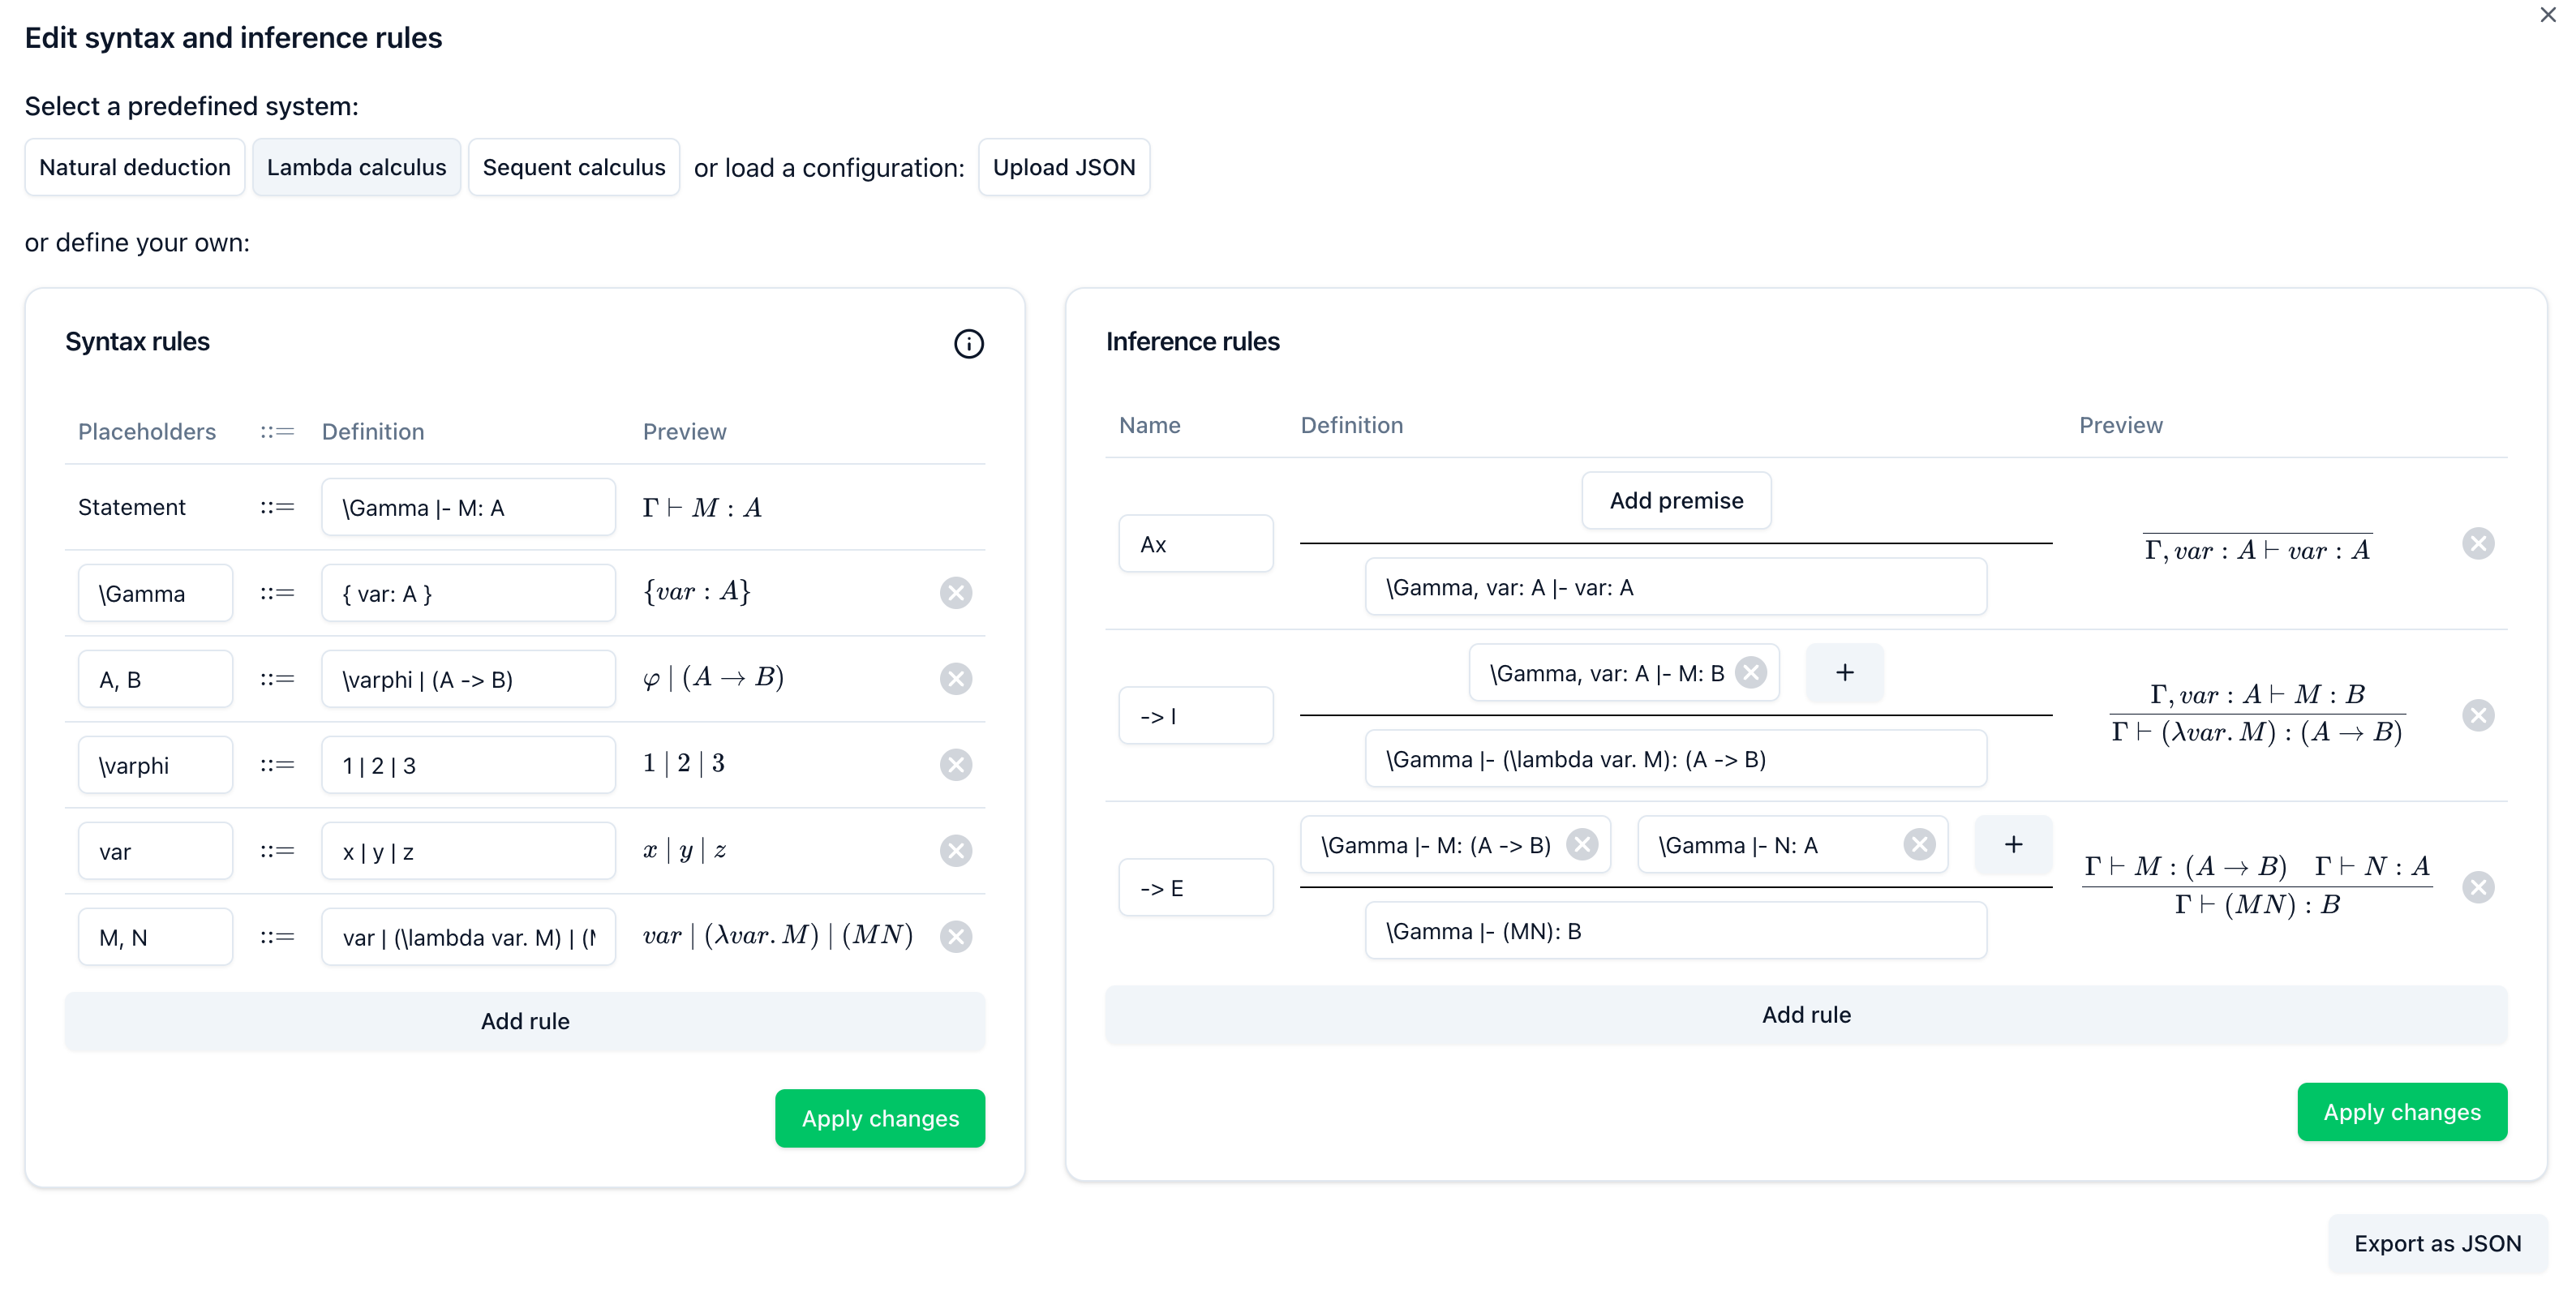
\includegraphics[width=\textwidth]{introduction/editor.png}
    \caption{Editing the proof system in \projectname{}}
    \label{fig:introduction:editor}
\end{figure}

\begin{figure}[!htbp]
    \centering
    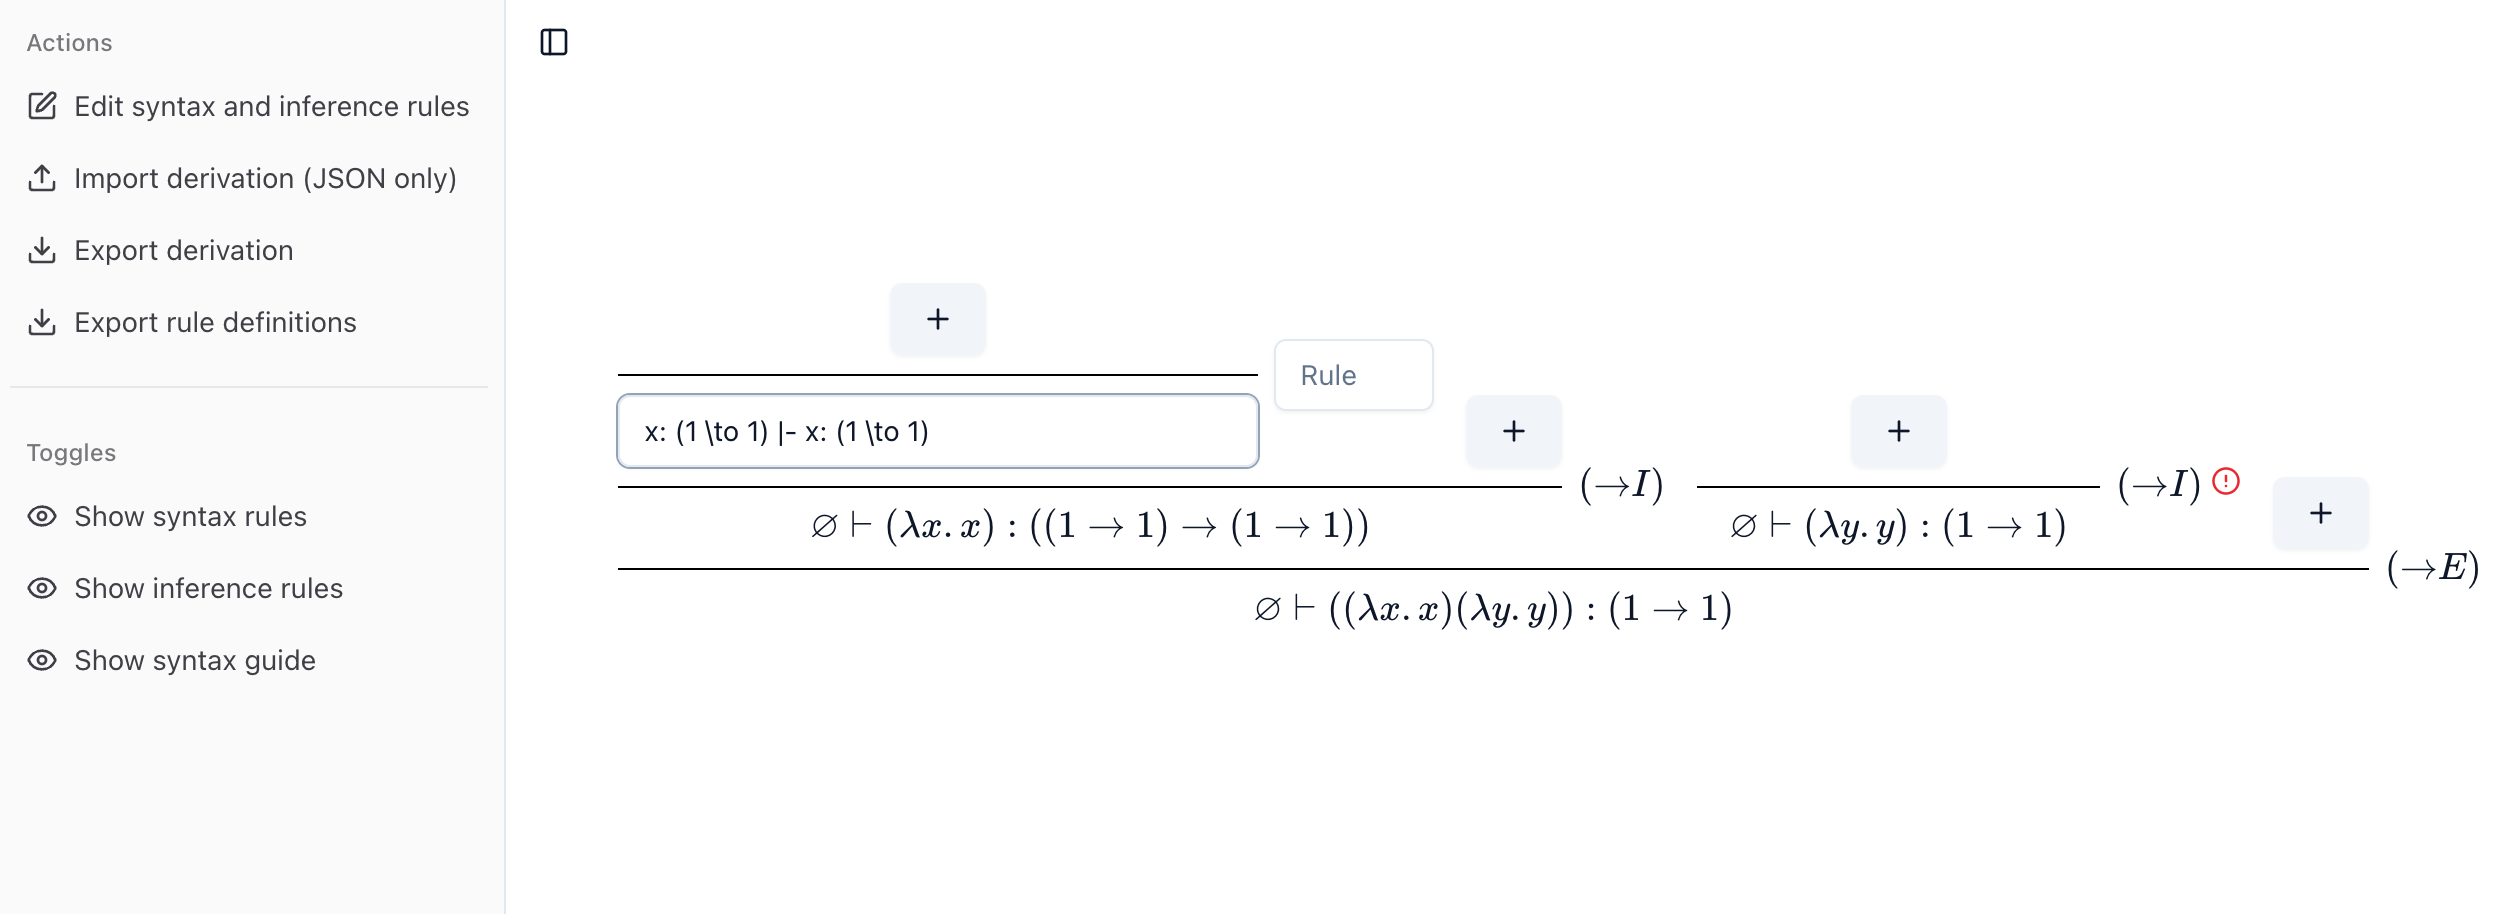
\includegraphics[width=\textwidth]{introduction/builder.png}
    \caption{Building a derivation in \projectname{}}
    \label{fig:introduction:builder}
\end{figure}
\chapter{Background}
This chapter provides an overview of the background knowledge necessary to understand the project.

\section{Lambda Calculus}
In the 1930s, Alonzo Church introduced the Lambda Calculus \cite{church:1936} as a model of computation that is Turing-complete \cite{turing:1937}. It is the basis of functional programming languages like Haskell, which all Computing students at Imperial are required to learn. In addition, the Lambda Calculus is taught as part of the mandatory second-year \textit{Models of Computation} module and the TSfPL elective. In this section, we will define $\lambda$-terms and the Curry type assignment system, then formulate alternative syntaxes in extended Backus-Naur form (EBNF) for constructing the relevant parsers.

\subsection{\(\lambda\)-terms}\label{lambda:lambda-terms}
\textit{$\lambda$-terms} are defined as follows \cite{church:1941}:
\[
    M,N \Coloneqq x \alt \underbracket[0.6pt]{(\lambda x. M)}_\text{abstraction} \alt \underbracket[0.6pt]{(MN)}_\text{application}
\]
where $x$ can be any symbol from an infinite list of term variables $a, b, c, \ldots, x, y, z \ldots$. Observe that abstractions and applications contain brackets to avoid ambiguity. We can alternatively express the syntax of $\lambda$-terms in Backus-Naur form (BNF):
\begin{align*}
    \nonterm{term} &\Coloneqq \nonterm{var} \alt \nonterm{abstraction} \alt \nonterm{application} \\
    \nonterm{var} &\Coloneqq \textit{any lowercase letter} \\
    \nonterm{abstraction} &\Coloneqq \term{(} \lambda \nonterm{var}. \nonterm{term} \term{)} \\
    \nonterm{application} &\Coloneqq \term{(} \nonterm{term} \nonterm{term} \term{)}
\end{align*}
While it is straightforward to parse $\lambda$-terms using this syntax, it may become inconvenient to write large $\lambda$-terms by hand, which is an important part of a student's learning experience. Therefore, we introduce the following conventions:
\begin{itemize}
    \item Applications are \textit{left-associative}, so $(MNP)$ is equivalent to $((MN)P)$.
    \item Outermost brackets can be dropped, so $\lambda x. x$ is equivalent to $(\lambda x. x)$.
    \item Repeated abstractions can be shortened, so $\lambda xyz. M$ is equivalent to $(\lambda x. (\lambda y. (\lambda z. M)))$.
\end{itemize}
We allow partial adherence to these conventions as students inexperienced with the $\lambda$ calculus may find additional brackets instructive, e.g. $\lambda x. ((\lambda x. x) y)$ drops the outermost brackets but not the brackets around the body of the abstraction. With these conventions in mind, we formulate a new syntax in Backus-Naur form:
\begin{align*}
    \nonterm{term} &\Coloneqq \nonterm{var} \alt \nonterm{unbracketed} \alt \nonterm{bracketed} \\
    \nonterm{var}  &\Coloneqq \textit{any lowercase letter} \\
    \nonterm{abstraction} &\Coloneqq \lambda \nonterm{var}. \nonterm{term} \\
    \nonterm{application} &\Coloneqq (\nonterm{application} \alt \nonterm{arg}) \nonterm{arg} \\
    \nonterm{arg} &\Coloneqq \nonterm{var} \alt \nonterm{bracketed} \\
    \nonterm{unbracketed} &\Coloneqq \nonterm{abstraction} \alt \nonterm{application} \\
    \nonterm{bracketed} &\Coloneqq \term{(} \nonterm{unbracketed} \term{)}
\end{align*}
Notice that the rule for $\nonterm{application}$ is left-recursive. This may cause infinite recursion in recursive descent parsers, which is certainly undesirable in a web application. We mitigate this by rewriting $\nonterm{application}$ in EBNF. The complete syntax of $\lambda$-terms with optional bracketing conventions in EBNF is presented here---the only change is made to the rule for $\nonterm{application}$.
\begin{align*}
    \nonterm{term} &\Coloneqq \nonterm{var} \alt \nonterm{unbracketed} \alt \nonterm{bracketed} \\
    \nonterm{var}  &\Coloneqq \textit{any lowercase letter} \\
    \nonterm{abstraction} &\Coloneqq \lambda \nonterm{var}. \nonterm{term} \\
    \nonterm{application} &\Coloneqq \nonterm{arg} \nonterm{arg} \{\nonterm{arg}\} \\
    \nonterm{arg} &\Coloneqq \nonterm{var} \alt \nonterm{bracketed} \\
    \nonterm{unbracketed} &\Coloneqq \nonterm{abstraction} \alt \nonterm{application} \\
    \nonterm{bracketed} &\Coloneqq \term{(} \nonterm{unbracketed} \term{)}
\end{align*}
Left-associativity of $\nonterm{application}$ will be enforced in the generation of the abstract syntax tree (AST).

\subsection{Curry types}\label{lambda:curry-types}
The set of Curry \textit{types} is defined as follows \cite{van-bakel:2022}:
\[
    A, B \Coloneqq \varphi \alt (A \rightarrow B)
\]
where $\varphi$ can be any symbol from an infinite list of type variables $\varphi_1, \varphi_2, \ldots$. When writing type variables by hand, it is often more convenient to use the subscript alone to represent a type variable, e.g. the type $((1 \rightarrow 2) \rightarrow 1)$ represents the type $((\varphi_1 \rightarrow \varphi_2) \rightarrow \varphi_1)$. We can express the syntax of Curry types in BNF:
\begin{align*}
    \nonterm{type} &\Coloneqq \nonterm{typevar} \alt \term{(} \nonterm{type} \rightarrow \nonterm{type} \term{)} \\
    \nonterm{typevar} &\Coloneqq \varphi_{\textit{any positive integer}}
\end{align*}
As with $\lambda$-terms, bracketing conventions are adopted for Curry types:
\begin{itemize}
    \item Arrow types are \textit{right-associative}, so $(1 \rightarrow 2 \rightarrow 1)$ is equivalent to $(1 \rightarrow (2 \rightarrow 1))$.
    \item Outermost brackets can be dropped, so $1 \rightarrow 2$ is equivalent to $(1 \rightarrow 2)$.
\end{itemize}
We reformulate the syntax of Curry types in BNF with optional bracketing conventions:
\begin{align*}
    \nonterm{type} &\Coloneqq \nonterm{typevar} \alt \nonterm{arrow} \\
    \nonterm{arrow} &\Coloneqq \nonterm{arg} \rightarrow \nonterm{arrow} \\
    \nonterm{arg} &\Coloneqq \nonterm{typevar} \alt \term{(} \nonterm{arrow} \term{)}
\end{align*}
We can rewrite the rule for $\nonterm{arrow}$ in EBNF as follows:
\begin{align*}
    \nonterm{type} &\Coloneqq \nonterm{typevar} \alt \nonterm{arrow} \\
    \nonterm{arrow} &\Coloneqq \nonterm{arg} \rightarrow \nonterm{arg} \{\rightarrow \nonterm{arg}\} \\
    \nonterm{arg} &\Coloneqq \nonterm{typevar} \alt \term{(} \nonterm{arrow} \term{)}
\end{align*}
As with $\lambda$-terms, the EBNF rule for $\nonterm{arrow}$ does not capture right-associativity, which can be handled when generating the AST.

\subsection{Type inference rules}\label{lambda:type-assignment}
$\lambda$-terms can be assigned types under Curry's type assignment system using the following derivation rules \cite{van-bakel:2022}:
\[
    (Ax): \frac{}{\Gamma, x:A \vdash x:A} \quad (\rightarrow I): \frac{\Gamma, x:A \vdash M:B}{\Gamma \vdash \lambda x. M: A \rightarrow B} \quad (\rightarrow E): \frac{\Gamma \vdash M: A \rightarrow B \quad \Gamma \vdash N: A}{\Gamma \vdash MN: A \rightarrow B}
\]
A \textit{context} $\Gamma$ is a set of statements in the form $x:A$, where $x$ is a variable and $A$ is a Curry type. All variables are assigned at most one type in any context, so $x:1, x:2$ is not a well-formed context since $x$ appears twice.

The syntax of a \textit{conclusion}\todo{Check with Steffen on terminology} in the form of $\Gamma \vdash M: A$ can be expressed in EBNF as follows:
\begin{align*}
    \nonterm{conclusion} &\Coloneqq \nonterm{context} \vdash \nonterm{term} : \nonterm{type} \\
    \nonterm{context} &\Coloneqq \varnothing \alt \nonterm{varassignment} \{, \nonterm{varassignment} \} \\
    \nonterm{varassignment} &\Coloneqq \nonterm{var} : \nonterm{type}
\end{align*}
where $\nonterm{term}$, $\nonterm{type}$, and $\nonterm{var}$ are taken from the syntax of $\lambda$-terms and Curry types.
\section{Milner's \textsc{ML}}
% type systems module, what is covered

\subsection{ML expressions}
ML expressions are defined as follows \cite{van-bakel:2022}:
\[
    E \Coloneqq x \alt c \alt (\lambda x. E) \alt (E_1 E_2) \alt (\texttt{let}\ x = E_1 \ \texttt{in}\  E_2) \alt (\texttt{fix}\ g. E)
\]
where $x$ represents term variables as in \ref{lambda:lambda-terms}, and $c$ can be any constant. In BNF:
\begin{align*}
    \nonterm{expr} &\Coloneqq \nonterm{var} \alt \nonterm{const} \alt \nonterm{abstraction} \alt \nonterm{application} \alt \nonterm{let} \alt \nonterm{fix} \\
    \nonterm{const} &\Coloneqq \textit{any constant} \\
    \nonterm{let} &\Coloneqq \term{(} \texttt{let}\ \nonterm{var} = \nonterm{expr}\ \texttt{in}\ \nonterm{expr} \term{)} \\
    \nonterm{fix} &\Coloneqq \term{(} \texttt{fix}\ \nonterm{var}. \nonterm{expr} \term{)}
\end{align*}
Bracketing conventions are the same as in \ref{lambda:lambda-terms}. We can trivially extend the EBNF syntax with bracketing conventions in \ref{lambda:lambda-terms} with the additional \textsc{ML} term constructs. The complete EBNF syntax is as follows:
\begin{align*}
    \nonterm{term} &\Coloneqq \nonterm{var} \alt \nonterm{unbracketed} \alt \nonterm{bracketed} \\
    \nonterm{var}  &\Coloneqq \textit{any lowercase letter} \\
    \nonterm{const} &\Coloneqq \textit{any constant} \\
    \nonterm{abstraction} &\Coloneqq \lambda \nonterm{var}. \nonterm{term} \\
    \nonterm{application} &\Coloneqq \nonterm{arg} \nonterm{arg} \{\nonterm{arg}\} \\
    \nonterm{let} &\Coloneqq \texttt{let}\ \nonterm{var} = \nonterm{expr}\ \texttt{in}\ \nonterm{expr} \\
    \nonterm{fix} &\Coloneqq \texttt{fix}\ \nonterm{var}. \nonterm{expr} \\
    \nonterm{arg} &\Coloneqq \nonterm{var} \alt \nonterm{const} \alt \nonterm{bracketed} \\
    \nonterm{unbracketed} &\Coloneqq \nonterm{abstraction} \alt \nonterm{application} \alt \nonterm{let} \alt \nonterm{fix} \\
    \nonterm{bracketed} &\Coloneqq \term{(} \nonterm{unbracketed} \term{)}
\end{align*}

\subsection{\textsc{ML} types}
\textsc{ML} types are defined as follows \cite{van-bakel:2022}:
\begin{align*}
    \sigma, \tau &\Coloneqq A \alt (\forall \varphi. \tau) \\
    A, B &\Coloneqq \varphi \alt c \alt (A \rightarrow B)
\end{align*}
where $c$ can be any type constant, e.g. \texttt{Int} and \texttt{Bool}. We develop a BNF syntax for \textsc{ML} types.
\begin{align*}
    \nonterm{type} &\Coloneqq \nonterm{basic} \alt \nonterm{quantified} \\
    \nonterm{basic} &\Coloneqq \nonterm{typevar} \alt \nonterm{typeconst} \alt \nonterm{arrow} \\
    \nonterm{typevar} &\Coloneqq \varphi_{\textit{any positive integer}} \\
    \nonterm{typeconst} &\Coloneqq \textit{any type constant} \\
    \nonterm{arrow} &\Coloneqq \term{(} \nonterm{basic} \rightarrow \nonterm{basic} \term{)} \\
    \nonterm{quantified} &\Coloneqq \term{(} \forall \nonterm{typevar}. \nonterm{type} \term{)}
\end{align*}
In addition to the bracketing conventions in \ref{lambda:curry-types}, we abbreviate quantified types like $(\forall \varphi_1. (\forall \varphi_2. \cdots (\forall \varphi_n. A) \cdots ))$ as $\forall \Vec{\varphi}. A$, where $\Vec{\varphi}$ represents a vector of type variables $\varphi_1, \ldots, \varphi_n$. We can also only drop brackets but not vectorise the type variables, so the same quantified type can be written as $\forall \varphi_1. \forall \varphi_2. \cdots \forall \varphi_n. A$. In practice, students of TSfPL rarely encounter quantified types with more than one bound type variable (i.e. $n > 1$), though such support may be beneficial regardless. Here, we allow mixing of type variables and vectors of type variables, so $\forall \varphi_1. \forall \Vec{\varphi}. \forall \varphi_2. A$ is well-formed.

We formalise the (optional) bracketing and abbreviation conventions in EBNF as follows:
\begin{align*}
    \nonterm{type} &\Coloneqq \nonterm{basic} \alt \nonterm{quantified} \\
    \nonterm{basic} &\Coloneqq \nonterm{typevar} \alt \nonterm{typeconst} \alt \nonterm{arrow} \\
    \nonterm{typevar} &\Coloneqq \varphi_{\textit{any positive integer}} \\
    \nonterm{typeconst} &\Coloneqq \textit{any type constant} \\
    \nonterm{typevec} &\Coloneqq \Vec{\varphi}_{\textit{any positive integer}} \\
    \nonterm{arrow} &\Coloneqq \nonterm{arg} \rightarrow \nonterm{arg} \{\rightarrow \nonterm{arg}\} \\
    \nonterm{arg} &\Coloneqq \nonterm{typevar} \alt \nonterm{typeconst} \alt \term{(} \nonterm{arrow} \term{)} \\
    \nonterm{quantified} &\Coloneqq \forall (\nonterm{typevar} \alt \nonterm{typevec}). \{\forall (\nonterm{typevar} \alt \nonterm{typevec}).\} \nonterm{type}
\end{align*}

\subsection{Type inference rules}
The derivation rules for types in \textsc{ML} are as follows:
\begin{center}
    \begin{minipage}{.4\textwidth}
        \begin{align*}
            (Ax) &: \frac{}{\Gamma, x: \tau \vdash x: \tau} \\[1em]
            (\rightarrow I) &: \frac{\Gamma, x: A \vdash E: B}{\Gamma \vdash \lambda x. E: A \rightarrow B} \\[1em]
            (let) &: \frac{\Gamma \vdash E_1: \tau \quad \Gamma, x: \tau \vdash E_2: B}{\Gamma \vdash \texttt{let}\ x = E_1\ \texttt{in}\ E_2: B} \\[1em]
            (\forall I) &: \frac{\Gamma \vdash E: \tau}{\Gamma \vdash E: \forall \varphi. \tau} (\text{$\varphi$ not in $\Gamma$})
        \end{align*}
    \end{minipage}%
    \begin{minipage}{.4\textwidth}
        \begin{align*}
            (\mathcal{C}) &: \frac{}{\Gamma \vdash c: vc} \\[1em]
            (\rightarrow E) &: \frac{\Gamma \vdash E_1: A \rightarrow B \quad \Gamma \vdash E_2: A}{\Gamma \vdash E_1 E_2: B} \\[1em]
            (fix) &: \frac{\Gamma, g: A \vdash E: A}{\Gamma \vdash \texttt{fix}\ g. E: A} \\[1em]
            (\forall E) &: \frac{\Gamma \vdash E: \forall \varphi. \tau}{\Gamma \vdash E: \tau \{A / \varphi\}}
        \end{align*}
    \end{minipage}
\end{center}
The syntax of conclusions in \textsc{ML} is essentially identical to that of the Lambda Calculus, where the rules for $\lambda$-terms and Curry types are replaced by those for \textsc{ML} terms and \textsc{ML} types, respectively.

\section{What makes a learning tool enjoyable to use?}
There are relatively few interactive learning tools for type systems compared to logic and natural deduction. This may be because most computer science students around the world are required to take courses on logic but not type systems \todo{citation needed}. At Imperial, all first-year undergraduate students in Computing and Joint Mathematics and Computing are required to study propositional logic and first-order logic, while Type Systems for Programming Languages (TSfPL) is an elective module offered from the third year onwards. In this section, we will discuss several learning tools for natural deduction in propositional and first-order logic, focusing on the features that make them enjoyable or not enjoyable to use.

\subsection{Pandora}
Pandora \cite{pandora:2007} is a tool that helps students learn Fitch-style natural deduction. The current version \cite{pandora} is written in Java by former Imperial students for their undergraduate capstone projects. At Imperial, it is presented during lectures in the first-year logic module.

\paragraph{Unnatural user interactions}
Using detailed logs to keep track of clicks and other interactions with Pandora, \cite{pandora:2007} found that students made infrequent use of the help and tutorial functionalities, even though they often failed to apply the rules correctly. For example, many students did not select the necessary lines before applying a rule. We hypothesise that students make these frequent mistakes when using Pandora because the sequence of interactions for applying rules does not correspond to how they apply natural deduction rules when writing proofs by hand. Suppose a student wants to apply the $\rightarrow I$ rule to lines 1 and 2. The justification would look like $\rightarrow I(1, 2)$. It is natural to write it from left to right, starting from $\rightarrow I$, then perhaps one or both of the brackets, then writing the line number 1, and finally the line number 2. The natural translation of this sequence into Pandora interactions would be to first click on the $\rightarrow I$ rule, then click on line 1, and finally click on line 2. Clearly, there is a discrepancy between this sequence and the current design.

Therefore, we should design our tool such that the interactions required to build derivations mimic as closely as possible how students would be producing assessed or marked work. The more similar they are, the less assistance and explanation is needed for students to use the tool correctly.

\paragraph{Installation necessary}
Pandora is \textit{not} a web-based application. It can be run either as a JAR executable or using Java Web Start, a deprecated framework for starting Java applications using a web browser. The former starts up but fails to start a proof correctly and is essentially useless. The latter is not supported from Java 11 onwards and the installation of supported Java versions can be extremely tedious, especially on machines not using Intel-based architectures, which are prevalent today \todo{citation needed}.

The current version of Pandora is written over two decades ago \todo{fact check}. No matter how carefully we choose our tech stack, we cannot guarantee how long native applications will work until it fails to be compatible with future hardware, or be as tedious to install for students two decades later as Pandora is today. A simple workaround is to build a web application. It does not require installation other than a suitable web browser and the current versions of the canonical web technologies---HTML, CSS, and JavaScript---should not cease to be forwards-compatible any time soon. \todo{citation needed}

\subsection{Carnap}
Carnap \cite{carnap:2018} is an educational tool for a variety of formal reasoning systems. It is written in Haskell and can be transpiled to JavaScript to be run on web browsers.

\section{How do interactive tools help students learn?}
\paragraph{Instant feedback}
Interactive tools provide instant feedback to students on the correctness of their proofs and derivations. Although lecturers can provide model answers to sample problems, there are often multiple correct solutions that would be tedious to exhaustively enumerate. Interactive tools ease the burden of teaching staff on verifying students' solutions. This is not to say they are unimportant in facilitating students' learning---they can help explain \textit{why} a proof or derivation is incorrect using various approaches \cite{nipkow:2012}; while interactive tools can also provide explanations to a certain degree, they are not necessarily tailored to the student's understanding.

\paragraph{More practice problems}
In the Department of Computing at Imperial, students are not provided with mark schemes or model answers to past papers. Although students have access to past paper solutions crowdsourced from seniors and former students, the solutions may not be complete or correct, especially for older papers. Students can use interactive tools to check their solutions, even in the lack of model answers. This extends beyond past papers at Imperial. Arbitrary new problems in natural deduction can be generated \cite{ahmed:2013} for as much practice as students want.

\paragraph{Enforcing methodical approaches}
Although students at Imperial who used Pandora scored similarly in the natural deduction parts of the final exam as those who did not use Pandora, the former approached the problems more methodically, were less likely to make arbitrary assumptions, and were more precise in their proofs \cite{pandora:2007}. This may be because Pandora makes it somewhat tedious to undo large parts of the proof by design. Even after adding the functionality to undo multiple proof steps as proposed in \cite{pandora:2007}, it is still more difficult than crossing out an erroneous solution on paper with a pen. This friction may prompt students to think more carefully before proceeding with the next proof step in Pandora, and with enough practice, on paper as well.

\section{Parsing inputs}
% Build parser using ts-parsec (use ts so everything runs on client-side)
% Allow a range of input formats (current: Haskell-like, future: latex, ascii?)
% Convert all input formats into latex


\chapter{User input}
\label{chapter:input}
This chapter describes the algorithms and data structures used for parsing and representing user input in \projectname{}. User input in \projectname{} can be divided into three categories: syntax rules (\Cref{section:syntax}), concrete terms (\Cref{section:term}), and inference rules (\Cref{section:inference}).
\section{Syntax rules}
\label{section:syntax}
Syntax rules define how well-formed input in a proof system should look like. Input that does not adhere to the syntax rules is considered nonsense and rejected by the system.

Users may want to extend pre-existing proof systems with new syntactic constructs, or even define a new proof system from scratch. \projectname{} provides an interface for modifying syntax rules, checks whether the syntax rules are defined sensibly, and verifies user input against an arbitrary set of syntax rules.

\Cref{syntax:syntax} defines the syntax in which a user expresses a syntax rule in \projectname{}. \Cref{syntax:parsing} describes the procedure for transforming an arbitrary set of syntax rules into intermediate internal representations, in preparation for verifying user input against the syntax rules.

\subsection{Syntax of syntax rules}
\label{syntax:syntax}
A syntax rule consists of:
\begin{itemize}
    \item a list of comma-separated \textbf{metavariables}, and
    \item a \textbf{definition}, consisting of one or more non-empty alternatives separated by vertical bars \lstinline{|}
\end{itemize}
In rule definitions, curly braces \lstinline|{}| represent a multiset. The structure of each element of a multiset is defined by the content enclosed within the curly braces. For example, the definition \lstinline|{ M: A }| represents a possibly empty collection of possibly duplicate elements following the structure \lstinline{M: A}.

Every valid syntax definition (i.e. collection of syntax rules) must contain at least one rule for a statement. All non-statement rules must specify metavariables. Otherwise, there is no way to refer to the definition of such rules and they might as well be removed from the syntax definition. Every syntax rule, including the rule defining a statement, can contain one or more non-empty alternatives.

The only special character in the definition of metavariables is the comma. The special characters in the definition of a syntax rule are the vertical bar \lstinline{|} and the curly braces \lstinline|{}|. Unlike in extended Backus-Naur form, characters like parentheses \lstinline{()} and brackets \lstinline{[]} do not carry any special meaning anywhere in this system and are no different from any other ordinary character. Certain groups of characters, such as \lstinline{|-} and \lstinline{->}, are treated as one symbol and shorthands for \LaTeX{} commands, such as \lstinline{\vdash} and \lstinline{\rightarrow}.

A rule definition can refer to itself or other rules by their metavariables. In the definition of syntax rules, there is no difference using one metavariable over another to refer to the same rule. For example, given the metavariables \lstinline{A} and \lstinline{B} for a rule, the definitions \lstinline{(A -> A)}, \lstinline{(B -> B)}, \lstinline{(A -> B)}, and \lstinline{(B -> A)} are all identical. However, it is useful to have multiple metavariables because in inference rules, metavariables are treated as names representing concrete objects.

\subsection{Parsing syntax rules}
\label{syntax:parsing}
The aim of this step is to generate a list of \lstinline{Token}s for each rule alternative, and thus a two-dimensional array of \lstinline{Token}s for each rule definition. These \lstinline{Token}s will be used to generate term parsers, i.e. parsers for parsing instances of each rule.

\subsubsection{Tokens}
The tokens are defined as follows:
\begin{itemize}
    \item \begin{lstlisting}[style=ds]
        class Terminal { constructor(readonly value: string) {} }
    \end{lstlisting}
    A \lstinline{Terminal} represents a string.
    \item \begin{lstlisting}[style=ds]
        class NonTerminal { constructor(readonly index: number) {} }
    \end{lstlisting}
    The \lstinline{index} field of \lstinline{NonTerminal} is the position of the rule referenced by the \lstinline{NonTerminal} in the ordered list of syntax rules. For example, if a syntax definition contains two rules
    \begin{align*}
        S &\Coloneqq \ldots \\
        A, B &\Coloneqq \ldots
    \end{align*}
    Then any occurrences of the metavariable $S$ are represented by a \lstinline{NonTerminal} with \lstinline{index} 0 and any occurrences of either of the metavariables $A$ or $B$ are represented by a \lstinline{NonTerminal} with \lstinline{index} 1.
    \item \begin{lstlisting}[style=ds]
        class Multiset { constructor(readonly tokens: Token[]) {} }
    \end{lstlisting}
    The \lstinline{tokens} field of \lstinline{Multiset} defines the structure of an element of the multiset. For example, consider a rule definition that contains a multiset:
    \begin{align*}
        S &\Coloneqq \{ var: A \}
    \end{align*}
    Assuming $var$ and $A$ are metavariables, the rule definition is represented by a \lstinline{Multiset} with the \lstinline{tokens} field set to \lstinline{[NonTerminal(...), Terminal(":"), NonTerminal(...)]}.
\end{itemize}
Finally, the \lstinline{Token} type is defined as
\begin{center}
    \lstinline*type Token = Terminal | NonTerminal | Multiset;*
\end{center}

\subsubsection{Procedure}
The process consists of three steps: splitting the metavariables and alternatives of the rule definitions, normalising them, and generating a parser for a rule alternative.

\paragraph{Splitting metavariables and alternatives of rule definitions}
When the backend receives user input from the frontend, every rule is specified by a string representing the metavariables and a string representing the definition. The metavariable string is split on commas to give a list of metavariables. To preprocess the definition string, all occurrences of \lstinline{|-} are replaced with \lstinline{\vdash}, the \LaTeX{} command for a turnstile, then the string is split on vertical bars \lstinline{|} to give a list of alternatives. The replacement is necessary and correct as \lstinline{|-} contains a vertical bar \lstinline{|} while \lstinline{\vdash} does not.

\paragraph{Normalise metavariables and rule definitions}
\label{syntax:normalise}
Aliases of a symbol are unified. For example, the symbol for an arrow \lstinline{->} can be represented by \lstinline{\rightarrow}, \lstinline{\to}, \lstinline{->}, and the Unicode character →. In this case, all aliases are replaced with \lstinline{->} (other than having the fewest characters and better readability, the choice is entirely arbitrary). Prior to the replacements, a space is added after all substrings that resemble a \LaTeX{} command, i.e. any substring beginning with \lstinline{\} and a string of non-whitespace characters. This ensures we do not accidentally replace parts of a \LaTeX{} command and e.g. turn \lstinline{\toI} into \lstinline{->I}. The user may have intended the latter, but the former is a typo nonetheless.

\paragraph{Generate parser}
The parser outputs three types of tokens: \lstinline{Terminal}, \lstinline{NonTerminal}, and \lstinline{Multiset}. The final parser tries to match a non-terminal, then (if it fails) a multiset, then (if both fail) a terminal. Each of these sub-parsers is generated as follows:
\begin{itemize}
    \item \lstinline{Terminal}: it matches, in descending order of priority, any string that resembles a \LaTeX{} command, any special group of characters e.g. \lstinline{|-} and \lstinline{->}, or any single character.
    \item \lstinline{NonTerminal}: it matches any metavariable across all rules in descending order of length.
    \item \lstinline{Multiset}: it matches a sequence of zero or more \lstinline{Terminal}s or \lstinline{NonTerminal}s enclosed within curly braces \lstinline|{}|. The empty multiset definition \lstinline|{}| is technically valid but not very useful: the user can only supply the empty set or a string of commas.
\end{itemize}

\subsection{Difficulty in left-factoring}
\label{syntax:factorisation}
\Cref{parsing:thenor} introduces the idiomatic and non-idiomatic ways of using the \lstinline{then} and \lstinline{or} combinators of \lstinline{parjs} together. The idiomatic approach requires the syntax definition to be left-factored. This section explains the difficulties of left-factoring syntax definitions, and therefore, why the idiomatic approach is not preferred.

\begin{definition}[First set]
    The \textit{first set} of a set of alternatives is the set containing every leading token of every alternative and the contributions of each of the leading tokens:
    \begin{itemize}
        \item If an alternative begins with a \lstinline{Terminal}, the contribution of the \lstinline{Terminal} to the first set is itself.
        \item If an alternative begins with a \lstinline{NonTerminal}, the contribution of the \lstinline{NonTerminal} to the first set is the first set of the rule corresponding to the \lstinline{NonTerminal}.
        \item If an alternative begins with a \lstinline{Multiset}, the contribution of the \lstinline{Multiset} to the first set is the union of the singleton \{ \textbackslash varnothing \} and the contribution of the first token of the element definition.
    \end{itemize}
\end{definition}

For example, consider the following syntax definition:
\begin{align*}
    \text{Statement} &\Coloneqq \Gamma \\
    \Gamma &\Coloneqq \{ A \} \\
    A &\Coloneqq x \alt y \alt z \alt (A \to A)
\end{align*}
The first set of each of the rules is computed as follows:
\begin{itemize}
    \item The first set of the rule corresponding to $A$ is the set containing $x$, $y$, $z$, and the left parenthesis $($.
    \item The first set of the rule corresponding to $\Gamma$ is the set containing \textbackslash varnothing and the contribution of $A$, i.e. the set containing $x$, $y$, $z$, and the left parenthesis $($.
    \item The first set of the rule corresponding to a statement is the contribution of $\Gamma$, i.e. the set containing \textbackslash varnothing, $x$, $y$, $z$, and the left parenthesis $($.
\end{itemize}

\subsubsection{\texorpdfstring{\lstinline{NonTerminal}}{NonTerminal}s sharing non-disjoint first sets with \texorpdfstring{\lstinline{NonTerminal}}{NonTerminal}s and \mbox{\texorpdfstring{\lstinline{Terminal}}{Terminal}s}}
\label{syntax:factorisation:nonterm}
Consider the following syntax definition:
\begin{align*}
    \text{Statement} &\Coloneqq Ax \alt By \\
    A &\Coloneqq x \alt Cz \alt z \\
    B &\Coloneqq x \alt y \alt w \\
    C &\Coloneqq y \alt w
\end{align*}
In the definition of the rule for a statement, the first set of the alternative $Ax$ is $\{ x, y, w, z \}$ while the first set of the alternative $By$ is $\{ x, y, w \}$. Since the first sets are not disjoint, the rule for a statement is not left-factored. One solution is to substitute the offending \lstinline{NonTerminal}s (in this case, $A$ and $B$) with their definitions and remove the rules for the \lstinline{NonTerminal}s if they are not used elsewhere:
\begin{align*}
    \text{Statement} &\Coloneqq xx \alt Czx \alt zx \alt xy \alt yy \alt wy \\
    C &\Coloneqq y \alt w
\end{align*}
After the substitution, the first set of the alternative $Czx$ is $\{ y, w \}$, which is not disjoint with the first sets of the alternatives $yy$ and $wy$. The offending \lstinline{NonTerminal} (in this case, $C$) can be substituted with its definition again:
\[
    \text{Statement} \Coloneqq xx \alt yzx \alt wzx \alt zx \alt xy \alt yy \alt wy
\]
Since there are no more \lstinline{NonTerminal}s left, left-factoring is straightforward:
\[
    \text{Statement} \Coloneqq x(x|y) \alt y(zx|y) \alt wzx \alt zx
\]
The main disadvantage of this approach is that information about the \lstinline{NonTerminal}s is destroyed by the substitutions. The parser generated from the left-factored definition after substitutions only treats the input as a list of \lstinline{Terminal}s, instead of a \lstinline{NonTerminal} followed by a \lstinline{Terminal}. This complicates the process of matching abstract terms in inference rules.

\subsubsection{\texorpdfstring{\lstinline{Multiset}}{Multiset}s sharing non-disjoint first sets with \texorpdfstring{\lstinline{NonTerminal}}{NonTerminal}s and \texorpdfstring{\lstinline{Terminal}}{Terminal}s}
Consider the following syntax definition:
\begin{align*}
    \text{Statement} &\Coloneqq \Gamma \vdash x \alt A \vdash y \\
    \Gamma &\Coloneqq \{ A \} \\
    A &\Coloneqq x \alt y \alt z \alt (A \to A)
\end{align*}
Humans reading the syntax definition can quickly differentiate the two alternatives of a statement by their last character: the term $x \vdash x$ should be parsed using the alternative $\Gamma \vdash x$ because the last character is $x$, while the term $x \vdash y$ should be parsed using the alternative $A \vdash y$ because the last character is $y$.

However, a parser does not know it should look for these defining characters in general. When the parser parses the term $x \vdash y$ from left to right, the prefix $x \vdash$ matches both alternatives: at this point, should the parser treat $x$ as a multiset with one element, a non-terminal, or an indeterminate form?

One attempt to parse correctly without regards to the the original structure of the definitions is to first rewrite the definition of the offending \lstinline{Multiset}s, then substitute occurrences of the \lstinline{Multiset}s with their rewritten definitions. In this example, the rule corresponding to $\Gamma$ is rewritten as
\[
    \Gamma \Coloneqq \varnothing \alt A \ [\text{optionally followed by 0 or more repetitions of },A]
\]
The offending occurrence of $\Gamma$ in the definition of a statement is substituted with its rewritten definition:
\begin{align*}
    \text{Statement} \Coloneqq \ &\varnothing \vdash x \\
    \alt &A \ [\text{optionally followed by 0 or more repetitions of },A] \vdash x \\
    \alt &A \vdash y
\end{align*}
The substituted definition of a statement can now be left-factored:
\begin{align*}
    \text{Statement} \Coloneqq \ &\varnothing \vdash x \\
    \alt &A \ [\text{optionally followed by 0 or more repetitions of },A] \vdash (x|y)
\end{align*}
This solution has the same drawback as that in \Cref{syntax:factorisation:nonterm}: the structure of $\Gamma$ is destroyed by rewriting and substitution. It is not always possible to determine whether the current part of the input is a \lstinline{NonTerminal} or a \lstinline{Multiset} before parsing the next part of the input (e.g. $x \vdash y$), which complicates attempts to recover the destroyed structure after fully parsing the input.

\subsubsection{\texorpdfstring{\lstinline{Multiset}}{Multiset}s sharing non-disjoint first sets with other \texorpdfstring{\lstinline{Multiset}}{Multiset}s}
Consider the following syntax definition:
\begin{align*}
    \text{Statement} &\Coloneqq \Gamma \vdash x \alt \Delta \vdash y \\
    \Gamma &\Coloneqq \{ Ax \} \\
    \Delta &\Coloneqq \{ By \} \\
    A &\Coloneqq x \alt y \\
    B &\Coloneqq x \alt z
\end{align*}

\subsection{Limitations}
\subsubsection{Metavariables cannot be used as terminals}
Suppose a user tries to define the syntax of $\lambda$-terms:
\begin{align*}
    M, N &\Coloneqq x \alt (\lambda x. M) \alt (MN) \\
    x &\Coloneqq x \alt y \alt z
\end{align*}
The second rule is necessary as the system does not ``know'' $x$ in the first rule is a variable: if a character is not a metavariable, it is treated as a \lstinline{Terminal}. However, contrary to what the user expects, the $x$ in the first alternative of the second rule is interpreted as a reference to its own rule. Since it is the first token of the alternative, the alternative is considered left-recursive by the parsing algorithm and causes the parsing algorithm to throw an error. The current workaround to this issue is as follows:
\begin{align*}
    M, N &\Coloneqq var \alt (\lambda var. M) \alt (MN) \\
    var &\Coloneqq x \alt y \alt z
\end{align*}
The use of $var$ is unconventional and differs from most textbook formulations. However, there is no good way to tell the parsing algorithm to treat $x$ as a literal string instead of a metavariable depending on where it appears. One solution is to treat lowercase metavariables as literal strings if it appears in the definition of its own rule and metavariables otherwise. However, this solution not only makes the system prejudiced against certain inputs, but is also equally problematic. A frustrated user may find the following definition of Curry types to be interpreted rather unexpectedly:
\[
  a, b \Coloneqq \varphi \alt (a \to b)
\]
\section{Concrete terms}
\label{section:term}
In this report, a \textit{concrete term} refers to an instance or realisation of a syntax rule in the derivation tree. A \textit{concrete term} can correspond to a Curry type, a $\lambda$-term, a multiset of propositional formulae, or any syntax rule defined by the user. For example, $((1 \to 2) \to 3)$ is a valid concrete term according to the rule $A \Coloneqq 1 \alt 2 \alt 3 \alt (A \to A)$, since it is a valid instance of the rule.

A \textit{concrete statement} is an instance or realisation of the syntax rule defining a statement.

A valid derivation tree consists of valid concrete statements and rule names. \projectname{} verifies whether each concrete statement conforms to the syntax rule defining a statement. This chapter describes the parsing algorithm that achieves this goal.

\subsection{Parsing concrete terms}
The aim of this step is to convert a term, given as a string, into a list of abstract syntax trees (ASTs). After parsing a syntax rule into \lstinline{Token}s, we generate a sub-parser for each \lstinline{Token} and combine the sub-parsers sequentially to form an overall parser. Each sub-parser outputs an AST, and the overall parser collects the ASTs from all sub-parsers into a list. The first AST is produced by the sub-parser corresponding to the first \lstinline{Token}, and so on.

\subsubsection{Abstract syntax trees (ASTs)}
The ASTs are defined as follows:
\begin{lstlisting}
    class TerminalAST { constructor(readonly value: string) {} }

    class NonTerminalAST {
        constructor(readonly index: number, readonly children: AST[]) {} }

    class MultisetAST { constructor(readonly elements: AST[][]) {} }

    type AST = TerminalAST | NonTerminalAST | MultisetAST;
\end{lstlisting}

\subsubsection{Procedure}
\label{term:procedure}
A list of \textit{delayed parsers} is generated using the \lstinline{later} combinator. A \textit{delayed parser}\footnote{In \lstinline{parjs}, a delayed parser has type \lstinline{DelayedParjser<T>}.} is a parser that does not carry any logic and must be initialised before being used for parsing \cite{parjs}. A delayed parser can be chained and combined with other parsers like a normal parser. There are two main benefits of generating delayed parsers and later initialising them:
\begin{itemize}
    \item It is possible to generate parsers for recursive rules. When generating the parser for a rule containing references to itself, the parser must be incomplete at any point of reference since the reference is part of the definition. A similar logic applies to mutually recursive rules.
    \item There is no need to devise an order in which the parsers for each rule is generated (e.g. by topologically sorting the references, such that every rule only references ``earlier'' rules whose parsers would have been all initialised). In fact, such an order or topological sort does not exist when there is recursion, since the reference graph contains cycles.
\end{itemize}
A term parser is generated by iterating over the tokens in every alternative of of the rule and examining the type of the token:
\begin{enumerate}
    \item \lstinline{Terminal}: parse the string verbatim.
    \item \lstinline{NonTerminal}: use the (delayed) parser corresponding to the rule number of the \lstinline{NonTerminal}.
    \item \lstinline{Multiset}: either parse the string \lstinline{\varnothing} (corresponding to the empty set) or a comma-separated list of one or more elements. To generate the parser for a multiset element, a parser is generated for each token of the element definition. Each of these parsers are chained together using the \lstinline{then} combinator.
\end{enumerate}
\chapter{Inference rules}
\label{chapter:inference}
\section{Syntax of inference rules}
An inference rule consists of:
\begin{itemize}
    \item A \textbf{name},
    \item One \textbf{conclusion} following the structure of a statement, and
    \item Zero or more \textbf{premises}, each following the structure of a statement
\end{itemize}
Inference rules are \textit{local}: checking whether an inference rule is applied correctly only requires information immediately above and below the step of applying the inference rule, but not any information further up or down the derivation tree.

\subsection{Inference rule terms and statements}
In this report, an \textit{inference rule statement} refers to one of the premises or the conclusion of an inference rule. A term appearing in an inference rule statement may not always be a valid term when given by the user. Consider the following syntax rule:
\[
    A, B \Coloneqq \varphi \alt (A \to B)
\]
In a derivation, the user can only input terms like $\varphi$, $(\varphi \to \varphi)$, and $((\varphi \to \varphi) \to \varphi)$. In an inference rule, however, an instance of a syntax rule can be represented by any of its placeholders and partially expanded versions of its definition. In this case, $A$, $B$, $(A \to B)$, $((A \to B) \to A)$, and even $((B \to \varphi) \to B)$ are all valid \textit{inference rule terms}. In this report, a \textit{(user-inputted) term} refers to an instance of a syntax rule that appears in derivations and an \textit{inference rule term} refers to an instance of a syntax rule that appears in an inference rule statement. All valid user-inputted are valid inference rule terms, and so the set of inference rule terms for any syntax definition with more than one non-statement rule is a strict superset of the set of user-inputted \textit{terms}\footnote{A syntax definition with only rules for statements does not have any placeholders, so the rule definitions cannot refer to any placeholders and must only consist of terminals and multisets. For such a syntax definition, the set of inference rule terms is equal to the set of terms.}.

\subsubsection{Placeholders in syntax rule definitions vs. inference rule statements}
Recall from \Cref{syntax:syntax} that in syntax rule definitions, placeholders for a rule can be used interchangeably. The following syntax rule is semantically identical to the example above:
\[
    A, B \Coloneqq \varphi \alt (A \to A)
\]
Even though $A$ appears twice in different positions of the same alternative, the two user-inputted terms that take their positions can be different. For example, $(\varphi \to (\varphi \to \varphi))$ is a valid instance of both versions of the syntax rule. However, the inference rule term $(A \to A)$ is compatible with a user-inputted term if and only if the two user-inputted sub-terms that take the positions of the two occurrences of $A$ are identical. In this case, $(\varphi \to (\varphi \to \varphi))$ is incompatible with the inference rule term $(A \to A)$ because the sub-terms $\varphi$ and $(\varphi \to \varphi)$ are different. The process of matching inference rule terms with user-inputted terms is explained in detail in \Cref{chapter:checking}.

\subsubsection{Multisets in inference rules}
\label{inference:multisets}
Consider the following syntax rules:
\begin{align*}
    \Gamma, \Delta &\Coloneqq \{ A \} \\
    A, B &\Coloneqq \varphi \alt (A \to B)
\end{align*}
On its own, $\Gamma$ represents a complete multiset. Now, consider the term $\Gamma, A$. $\Gamma$ represents a multiset with one element removed. The removed element is given the name $A$. Since an element can be removed, the user-inputted multiset must contain at least one element: trying to match the user-inputted term $\varnothing$ against the inference rule term $\Gamma, A$ results in an error. Note that $\Gamma$ can be empty. Analogously, it is possible to:
\begin{itemize}
    \item Match multiple multiset elements, such as $\Gamma, A, B$ and $\Gamma, A, A, A$.
    \item Match multiple multisets, such as $\Gamma, \Delta$.
    \item Match multiple multisets and multiset elements, such as $\Gamma, \Delta, A, B$.
\end{itemize}

It is also possible to match multiset elements with specific structures. The following are all valid inference rule terms:
\[
    \Gamma, (A \to B) \qquad \Gamma, (A \to (A \to A)) \qquad \Gamma, ((\varphi \to B) \to A)
\]
since $(A \to B)$, $(A \to (A \to A))$, and $((\varphi \to B) \to A)$ are all valid expansions of the definition of the second syntax rule, of which $A$ is a placeholder.

The order of the multiset placeholders and multiset element placeholders does not matter. This means a multiset term is identical to any of its permutations. The following terms are all identical:
\[
    \Gamma, \Delta, A, B \qquad \Gamma, B, \Delta, A \qquad A, B, \Delta, \Gamma \qquad \Delta, B, A, \Gamma \qquad \ldots
\]

Note that a placeholder (in this case, $\Gamma$ or $\Delta$) can represent a multiset if and only if at least one of its alternatives only consists of a multiset and no other tokens. For example, if the first syntax rule in the example above is changed to
\[
    \Gamma, \Delta \Coloneqq \{ A \}: B
\]
instead, things like $\Gamma, A$ and $\Gamma, \Delta, A$ are not valid inference rule terms for the modified syntax rule. 
\section{User interface}

\section{Parsing inference rules}
The aim of this step is to generate parsers for parsing an inference rule statement into a list of \lstinline{Matchable} tokens.

\subsection{\texorpdfstring{\lstinline{Matchable}}{Matchable} tokens}
\lstinline{Matchable} tokens are to inference rules like ASTs are to terms and \lstinline{Token}s are to syntax rules. \lstinline{Matchable} tokens represent the structure of an inference rule statement. They are defined as follows:
\begin{lstlisting}
    class MatchableTerminal { constructor(readonly value: string) {} }

    class Name { constructor(readonly index: number, readonly name: string) {} }

    class MatchableNonTerminal {
        constructor(readonly index: number, readonly children: Matchable[]) {} }

    class MultisetElement { constructor(readonly tokens: Matchable[]) {} }

    class MatchableMultiset {
        constructor(
            readonly index: number,
            readonly elements: (Name | MultisetElement)[]
        ) {}
    }

    type Matchable = MatchableTerminal | Name | MatchableNonTerminal | MatchableMultiset;
\end{lstlisting}
The semantics of the \lstinline{Matchable} tokens are as follows:
\begin{itemize}
    \item \lstinline{MatchableTerminal}: match the string stored in the \lstinline{value} field.
    \item \lstinline{Name}: assign exactly one AST to \lstinline{name} and ensure this assignment is compatible with all other occurrences of the same \lstinline{name} in other statements of the same inference rule. The AST must represent an instance of the syntax rule at \lstinline{index}\footnote{The \lstinline{index} field can be deduced from the \lstinline{name} field since the placeholders are unique across all syntax rules. The \lstinline{index} field exists merely to simplify bookkeeping.}.
    \item \lstinline{MatchableNonTerminal}: match an inference rule term corresponding to the syntax rule at \lstinline{index}. The structure of the inference rule term is given by the \lstinline{children} field.
    \item \lstinline{MatchableMultiset}: match a multiset of elements given by the \lstinline{elements} field. A member of \lstinline{elements} can either be a \lstinline{Name} or a \lstinline{MultisetElement}. A \lstinline{Name} refers to a multiset (e.g. $\Gamma$ and $\Delta$ in the example in the previous section) while a \lstinline{MultisetElement} refers to a multiset element that must be matched from the user-inputted multiset term (e.g. $A$ and $(A \to B)$ in the previous section). The \lstinline{elements} field is represented as an (ordered) array instead of an unordered set purely for simpler bookkeeping in the matching algorithm.
\end{itemize}
\subsection{Procedure}
Parsing inference rule statements is extremely similar to parsing terms, as an inference rule statement can be thought of as an instance of a statement in a different context. As with generating term parsers, a delayed parser is created  for every syntax rule using the \lstinline{later} combinator. Each of these delayed parsers is instantiated by iterating over the tokens in every alternative of the syntax rule and examining the type of the token:
\begin{itemize}
    \item \lstinline{Terminal}: parse the string verbatim and wrap the result in a \lstinline{MatchableTerminal} token.
    \item \lstinline{NonTerminal}: either parse a placeholder of the rule corresponding to the rule number (i.e. the \lstinline{index} field of the \lstinline{NonTerminal}), or an expanded version of the definition of the syntax rule using the (delayed) parser corresponding to the rule. The former produces a \lstinline{Name} token while the latter produces a \lstinline{MatchableNonTerminal} token.
    \item \lstinline{Multiset}: either parse \lstinline{\varnothing} (corresponding to the empty set) or a comma-separated list of multiset elements, as described in \Cref{inference:multisets}. If placeholders for multisets are applicable here (i.e. the \lstinline{Multiset} token is the only token of an alternative of the syntax rule definition, and the syntax rule does not define a statement), the comma-separated list can contain both individual multiset elements and placeholders for multisets. Since the \lstinline{Multiset} token does not store the rule number of the rule it is part of, the rule number is passed as an argument to the function which generates inference rule parsers.
\end{itemize}
\chapter{Rule checking}
\label{chapter:checking}
As the user builds the derivation tree, the application checks whether the inference rules are applied correctly and whether the derivation is complete and correct. Since the application only supports \textit{localised} inference rules, it suffices to check at every dividing line of the derivation tree, whether the user-inputted premises immediately above the line and the user-inputted conclusion immediately below the line are compatible with the inference rule specified by the user-inputted rule name. A derivation is complete and correct if and only if all inference rules in the derivation are compatible with the user input.

An inference rule is compatible with the user input if and only if there is a mapping of names (i.e. metavariables) to ASTs such that replacing all the names in the inference rule with the corresponding ASTs according to the mapping gives the user input. There can be many such mappings for a given inference rule and user input. Since the inference rules are localised, each mapping only applies to one application of an inference rule and need not apply to the rest of the derivation.

\Cref{checking:matching} describes the procedure for obtaining a mapping of names to ASTs given a user-inputted statement and the structure of the corresponding inference rule statement. \Cref{checking:verifying} describes how the procedure described in \Cref{checking:matching} is used to check whether all user-inputted premises and the user-inputted conclusion are compatible with the inference rule.

\section{Matching}
\label{checking:matching}
The aim of this step is to produce a mapping of names to ASTs. Matching is done individually to every inference rule statement.

\subsection{Inputs and outputs of the matching algorithm}
The matching algorithm takes in two mappings as arguments and modifies them in place. The two mappings are:
\begin{itemize}
    \item \lstinline{names}: a mapping where each entry maps a name (as a string) to an AST. A name \textit{must} be mapped to the AST according to \lstinline{names} if the inference rule is applied correctly.
    \item \lstinline{unmatchedPossibilities}: a mapping where each entry maps a name (as a string) that does not appear in \lstinline{names} to a set of ASTs. A name \textit{can} be mapped to any AST in the set according to \lstinline{unmatchedPossibilities} if the inference rule is applied correctly, yet it is not known which of the ASTs the name will ultimately end up getting mapped to at the time of matching.
\end{itemize}
The matching algorithm checks whether the mappings deduced from the user input and the structure of the inference rule statement are consistent with \lstinline{names} and \lstinline{unmatchedPossibilities}, and throws an error whenever it first finds an inconsistency.

\subsection{Procedure outline}
\label{matching:procedure}
\begin{enumerate}
    \item Parse the user-inputted statement into a list of ASTs.
    \item Check the list of ASTs has the same length as the list of \lstinline{Matchable} tokens in the inference rule statement.
    \item Pair up each AST with the corresponding \lstinline{Matchable} token and recursively match each pair.
    \item Repeat step 3 until no new names are added to \lstinline{names}.
\end{enumerate}
Step 3 is repeated because the mappings generated by matching the ASTs further down the list may imply mappings that could not be deduced in an earlier pass. Consider the conclusion of the action rule in natural deduction $\Gamma, A \vdash A$ and the user input $x, y \vdash y$. Suppose the ASTs and \lstinline{Matchable} tokens are matched from left to right starting with \lstinline{names} empty. Step 3 above can be broken down into the following smaller steps:
\begin{enumerate}
    \item Match $x, y$ with $\Gamma, A$. Since there are no existing mappings, $A$ can either be mapped to $x$ or $y$ and $\Gamma$ can either be mapped to the multiset containing $y$ or the multiset containing $x$.
    \item Match $\vdash$ with $\vdash$.
    \item Match $y$ with $A$. Clearly, $A$ must be mapped to $y$. This mapping is stored in \lstinline{names}.
\end{enumerate}
In the second iteration of step 3, when trying to match $x, y$ with $\Gamma, A$ again, the mapping of $A$ to $y$ implies the mapping of $\Gamma$ to the multiset containing $x$. This deduction could not be made in the first iteration.

The subsequent subsections explain step 3 in greater detail. From this point onwards, \lstinline{ast} and \lstinline{token} refer to the AST and the \lstinline{Matchable} token that are being matched, respectively.

\subsection{Matching a \texorpdfstring{\lstinline{TerminalAST}}{TerminalAST}}
Matching succeeds if and only if \lstinline{token} is a \lstinline{MatchableTerminal} containing the same string as \lstinline{ast}.

\subsection{Matching a \texorpdfstring{\lstinline{NonTerminalAST}}{NonTerminalAST}}
If \lstinline{token} is neither a \lstinline{Name} or a \lstinline{MatchableNonTerminal}, matching fails. Otherwise, if \lstinline{token} is a:
\begin{itemize}
    \item \lstinline{Name}: if the name is in \lstinline{names}, matching succeeds if and only if the mapped AST (i.e. \lstinline{names[name]}) is the same as \lstinline{ast}. Otherwise, create a new mapping from the name to \lstinline{ast}.
    \item \lstinline{MatchableNonTerminal}: if either of the following does not hold, matching fails:
    \begin{itemize}
        \item \lstinline{ast.index} is equal to \lstinline{token.index}. In other words, the rule number of \lstinline{ast} is the same as the rule number of \lstinline{token}.
        \item \lstinline{ast.children} has the same length as \lstinline{token.children}. In other words, there are as many children ASTs representing the structure of \lstinline{ast} as there are children \lstinline{Matchable} tokens representing the structure of \lstinline{token}.
    \end{itemize}
    If both of the above are true, pair up each child AST with the corresponding child \lstinline{Matchable} token and recursively match each pair, like in step 3 of \Cref{matching:procedure}.
\end{itemize}
\subsection{Matching a \texorpdfstring{\lstinline{MultisetAST}}{MultisetAST}}
If \lstinline{token} is not a \lstinline{MatchableMultiset}, matching fails. Otherwise, split up the \lstinline{elements} field of \lstinline{token} (which has type \lstinline{(Name | MultisetElement)[]}) into \lstinline{Name}s and \lstinline{MultisetElement}s.

For every \lstinline{Name} in \lstinline{token.elements}:
\begin{itemize}
    \item If the name is in \lstinline{names} (i.e. it is already mapped to an AST), check the mapped AST (i.e. \lstinline{names[name]}) has type \lstinline{MultisetAST}. Remove all elements in the mapped AST from \lstinline{ast.elements}. If any element in the mapped AST cannot be found in \lstinline{ast.elements}, throw an error.
    \item Otherwise, matching is postponed.

\end{itemize}

For every \lstinline{MultisetElement} in \lstinline{token.elements}, find all \textit{actual elements} (i.e. an element of \lstinline{ast.elements} with type \lstinline{AST[]}) that are compatible with the \lstinline{MultisetElement}. The procedure for finding compatible actual elements will be described in the next subsection.
\begin{itemize}
    \item If there are no matches, i.e. none of the actual elements are compatible with the \lstinline{MultisetElement}, throw an error.
    \item If there is exactly one match, i.e. exactly one actual element is compatible with the \lstinline{MultisetElement}, match the actual element with the \lstinline{MultisetElement}.
    \item If there are at least two matches, postpone the matching and update \lstinline{unmatchedPossibilities} as follows:
    \begin{enumerate}
        \item For every actual element that is compatible with the \lstinline{MultisetElement}, assume the \lstinline{MultisetElement} should be mapped to the actual element and generate a mapping where each entry maps a name in the \lstinline{MultisetElement} to an AST.
        \item For every name in the \lstinline{MultisetElement} but not in \lstinline{names} (i.e. it has not been mapped to an AST for certain), if it exists in \lstinline{unmatchedPossibilities}, update the corresponding entry as follows:
        \begin{center}
            \lstinline|unmatchedPossibilities[name] = { names1[name], names2[name], ... } $\cap$ unmatchedPossibilities[name]|
        \end{center}
        where \lstinline{names1}, \lstinline{names2}, etc. are the mappings generated from the previous step. Otherwise, if the name does not exist in \lstinline{unmatchedPossibilities}, create a new entry in \lstinline{unmatchedPossibilities} as follows:
        \begin{center}
            \lstinline|unmatchedPossibilities[name] = { names1[name], names2[name], ... }|
        \end{center}
    \end{enumerate}
\end{itemize}

\subsubsection{Finding actual elements compatible with a \texorpdfstring{\lstinline{MultisetElement}}{MultisetElement}}
Create an empty set of possibilities. For every actual element remaining in the user-inputted multiset (i.e. after all multiset names are matched and the elements in the mapped AST are removed from \lstinline{ast.elements}):
\begin{enumerate}
    \item Check the actual element (which has type \lstinline{AST[]}) has the same length as the \lstinline{children} field of the \lstinline{MultisetElement}. In other words, check there are as many children ASTs representing the structure of the actual element as there are children \lstinline{Matchable} tokens representing the structure of the \lstinline{MultisetElement}.
    \item Check the actual element is not already in the set of possibilities. Recall the aim of finding compatible actual elements is to determine whether the \lstinline{MultisetElement} can be matched with an actual element with certainty. If the \lstinline{MultisetElement} is compatible with multiple identical actual elements, there is no difference between matching the \lstinline{MultisetElement} with one of the duplicates and matching it with any of the other duplicates, since any modifications to \lstinline{names} will be identical.
    \item Make a shallow copy of \lstinline{names}. The copy is a new mapping from names (as strings) to ASTs where the ASTs share the same references as in \lstinline{names}. Assigning a new name or removing an existing name of the shallow copy will not affect \lstinline{names}, but modifying any of the ASTs will cause the same changes in \lstinline{names}. A shallow copy is acceptable since the matching algorithm only adds names to \lstinline{names} and never modifies the ASTs in place.
    \item Pair up each AST in the actual element with the corresponding \lstinline{Matchable} token of the \lstinline{MultisetElement}. Try to match each (AST, \lstinline{Matchable}) pair using the shallow copy of \lstinline{names}. A shallow copy of \lstinline{names} instead of \lstinline{names} is used because the matching may fail. The matching algorithm assumes the given AST \lstinline{must} be compatible with the given \lstinline{Matchable} token, so any error thrown indicates the user input is incorrect. This assumption is reasonable when matching at the top level, i.e. matching the user input with the structure of the inference rule statement, but less so when matching is used as a means to explore possibilities.
    \item If the matching succeeds, add the actual element to the set of possibilities.
\end{enumerate}

\section{Verifying}
\label{checking:verifying}
The aim of this step is to verify whether an inference rule is applied correctly by the user.

\subsection{Procedure outline}
Given a string representing the user-inputted conclusion, a list of strings representing the user-inputted premises, and the parsed inference rule, the verification algorithm is as follows:
\begin{enumerate}
    \item Check the user has given the same number of premises as defined in the inference rule.
    \item Repeat the following steps until no new names are added:
    \begin{enumerate}
        \item Match the user-inputted conclusion with the structure of the conclusion as defined by the inference rule.
        \item Match each user-inputted premise with the structure of the corresponding premise as defined by the inference rule.
    \end{enumerate}
    Here, the order of matching the abstract statements is arbitrary. Without analysing the structure of the inference rule, any matching order~ when given an arbitrary inference rule works equally well, since the matching algorithm is idempotent. For example, it is equally effective to match the premises before the conclusion or to match the premises in a random order. The matching steps are repeated for a similar reason as repeating step 3 in \Cref{matching:procedure}: matching a later inference rule statement may give more information for generating additional mappings when re-matching an earlier inference rule statement that cannot be generated on an earlier iteration.
    \item If \lstinline{unmatchedPossibilities} is empty, verification succeeds if and only if none of the matching steps throws any errors.
    \item Otherwise, recursively explore all possible assignments of names to ASTs. Verification succeeds if and only if there is at least one assignment that does not result in any error when parsing.
\end{enumerate}
\chapter{Evaluation}
\projectname{} should be both reliable and intuitive to use. Here, reliability means the application correctly verifies a derivation if and only if the derivation is correct. If the application is not reliable, users may want to double-check their derivation by other means. If the application is not intuitive, users may need to spend more time learning how to use it. In both cases, users experience more friction and waste time on using the application, making the application less appealing than its humble competitor: pen and paper.

\Cref{evaluation:correctness} describes how the algorithms are tested and refined to support a large range of proof systems. \Cref{evaluation:ux} discusses how user testing is done to evaluate the intuitiveness of \projectname{}, the findings of user testing, and the improvements made to address these findings.

\section{Correctness of algorithms}
\label{evaluation:correctness}
The correctness of the parsing, matching, and verification algorithms are verified using unit tests. Some test cases are based on the three pre-defined proof systems---Natural Deduction \ndt{}, Curry type assignment for the $\lambda$-calculus, and the system \textsc{lk}---while other test cases are based on variously modified rules from these systems and designed to catch edge cases. Some test cases based on the $\lambda$-calculus are taken from the course notes for the Type Systems for Programming Languages module at Imperial \cite{van-bakel:2022}. Some test cases based on the system \textsc{lk} are taken from a set of online logic notes \cite{sequent}.

There is a high degree of confidence in the matching and verification algorithms, since they are based on custom data structures independent of the user input. To identify further edge cases in the parsing algorithm and determine how well the parsing algorithm adapts to a wide range of user inputs, the parsing algorithm is tested against extensions of the pre-defined systems and brand new proof systems.

\subsection{\lc{} with pairs}
\label{evaluation:lambda-pairs}
\begin{definition}[$\lambda$-terms and Curry types]
    The syntaxes of $\lambda$-terms and Curry types are extended with the following constructors \cite{van-bakel:2022}:
    \begin{align*}
        M, N &\Coloneqq \ldots \alt \langle M, N \rangle \alt \textsf{left}(M) \alt \textsf{right}(M) \\
        A, B &\Coloneqq \ldots \alt (A \times B)
    \end{align*}
\end{definition}
\begin{definition}[Type assignment rules]
    The three new constructors for $\lambda$-terms are accompanied by the following extensions to the type assignment rules:
    \[
        (\textsf{Pair}): \frac{\Gamma \vdash M: A \quad \Gamma \vdash N: B}{\Gamma \vdash \langle M, N \rangle: (A \times B)} \quad (\textsf{left}): \frac{\Gamma \vdash M: (A \times B)}{\Gamma \vdash \textsf{left}(M): A} \quad (\textsf{right}): \frac{\Gamma \vdash M: (A \times B)}{\Gamma \vdash \textsf{right}(M): B}
    \]
\end{definition}
Although the user can type ``left'' and ``right'' for the two constructors, they will be rendered in math mode in \LaTeX{} as $left$ and $right$, which do not look the nicest. Prior to testing with the $\lambda$-calculus with pairs, the parsing algorithm can only handle \LaTeX{} commands that do not take any arguments, such as ``\textbackslash Gamma'' for $\Gamma$ and ``\textbackslash varphi'' for $\varphi$. The $\lambda$-calculus with pairs motivates extending the parsing algorithm to parse \LaTeX{} commands as literal strings. In this case, ``\lstinline|\textsf{left}(M)|'' should be rendered as $\textsf{left}(M)$ and parsed into \lstinline{Token}s as
\begin{center}
    \lstinline|[Terminal("\textsf{left}"), Terminal("("), NonTerminal(...), Terminal(")")]|
\end{center}
\Cref{fig:evaluation:lambda-with-pairs-definition} shows the definitions of syntax and inference rules in \projectname{}. \Cref{fig:evaluation:lambda-with-pairs-derivation} shows a derivation which uses all three new type assignment rules.
\begin{figure}[!htbp]
    \centering
    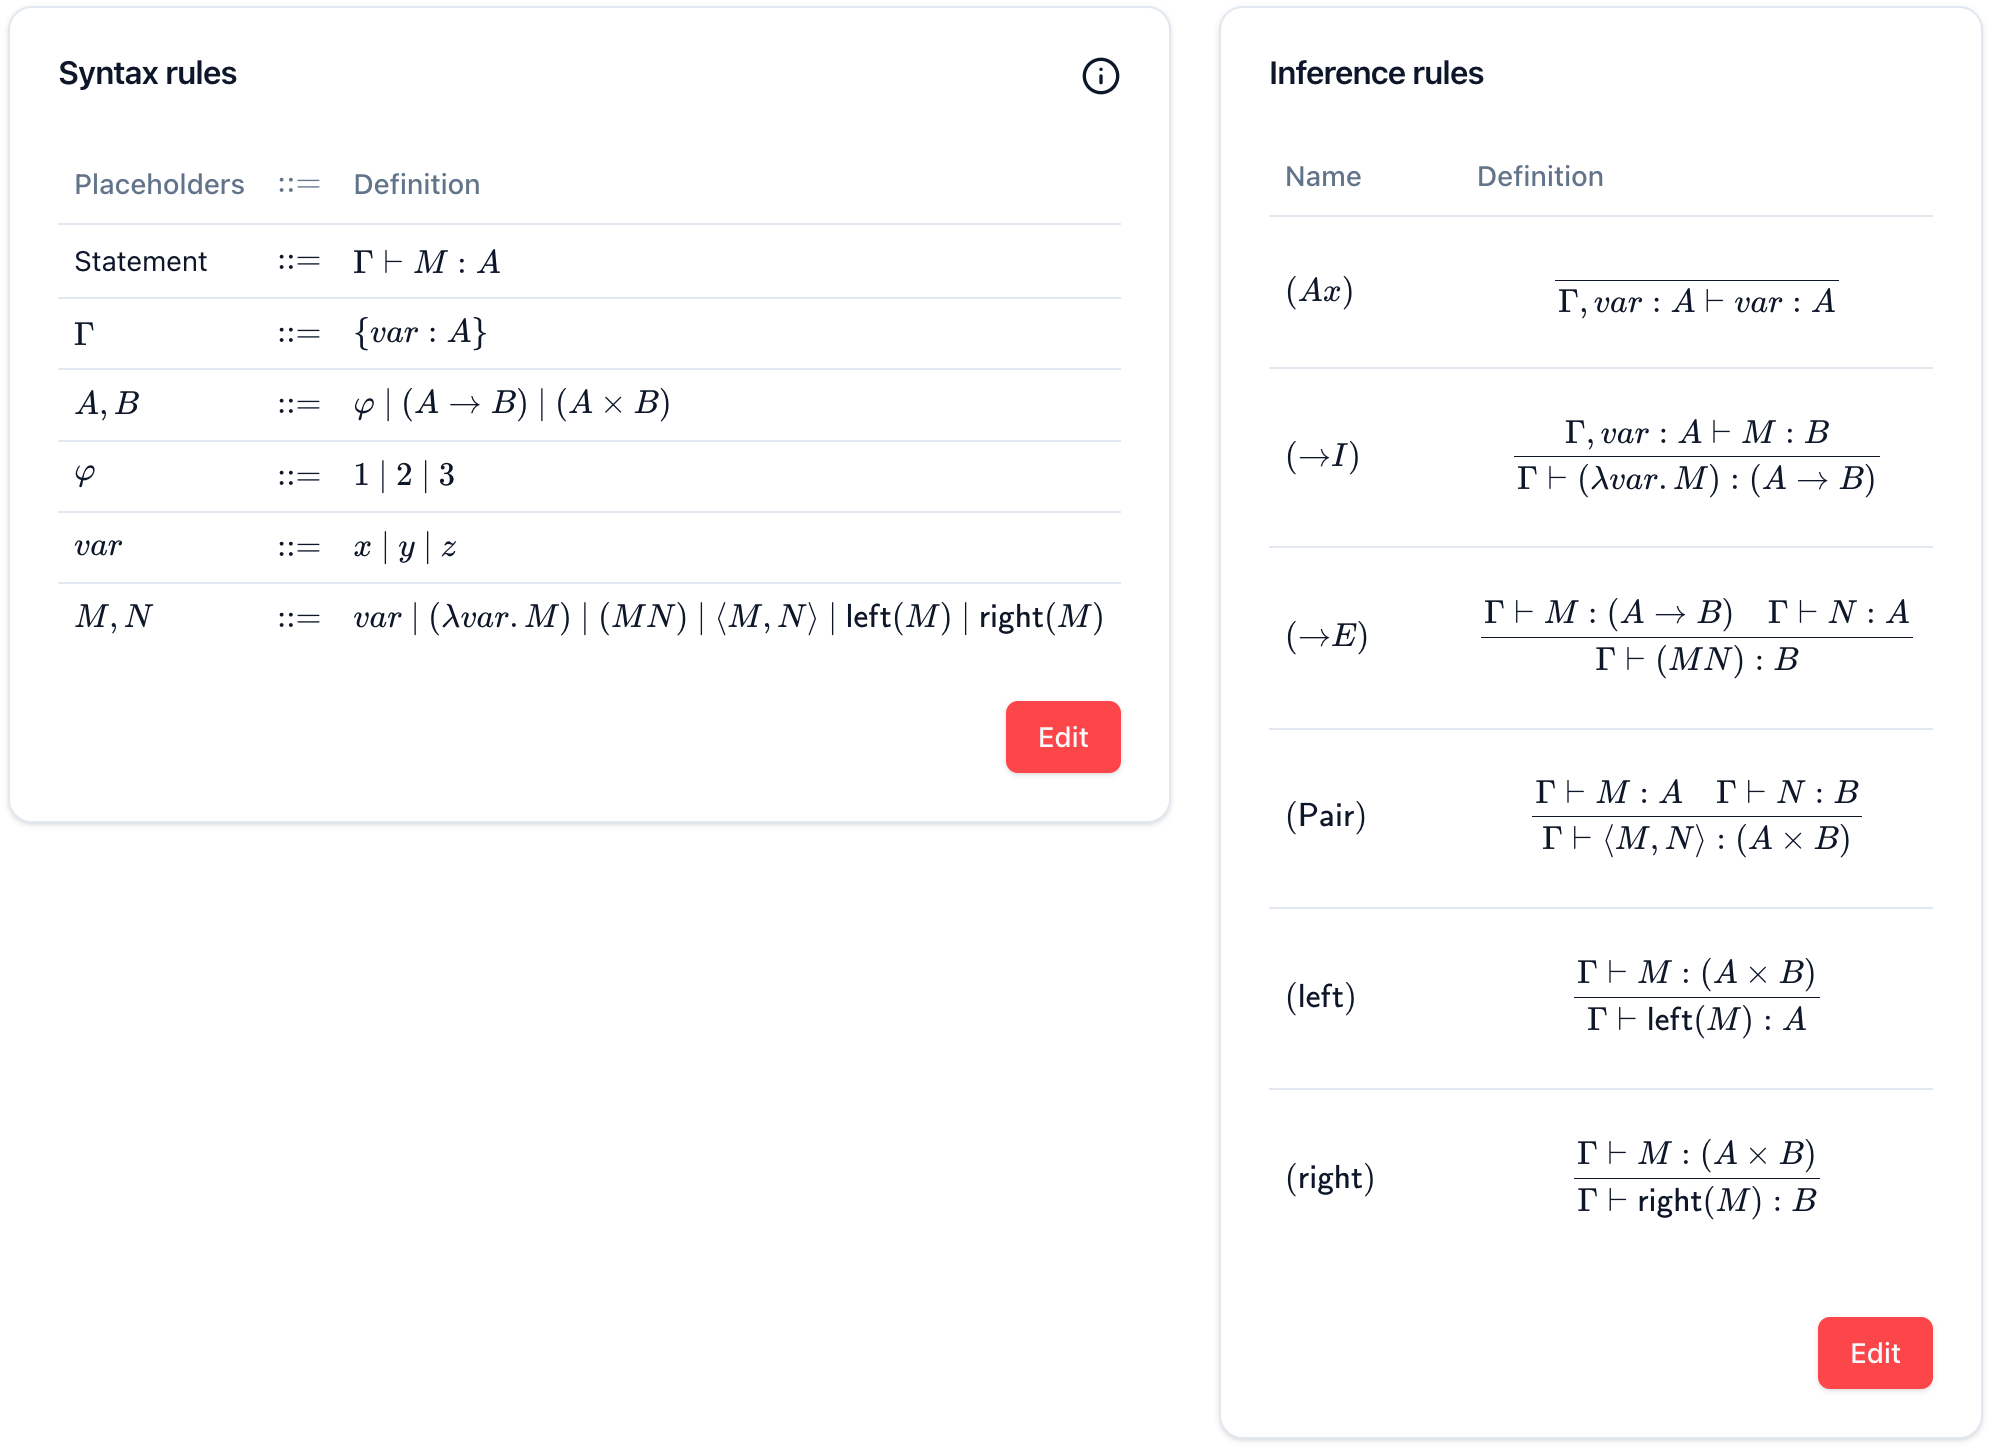
\includegraphics[width=\textwidth]{evaluation/lambda-with-pairs-definition.png}
    \caption{Definition of syntax and inference rules of $\lambda$-calculus with pairs in \projectname{}}
    \label{fig:evaluation:lambda-with-pairs-definition}
\end{figure}
\begin{figure}[!htbp]
    \centering
    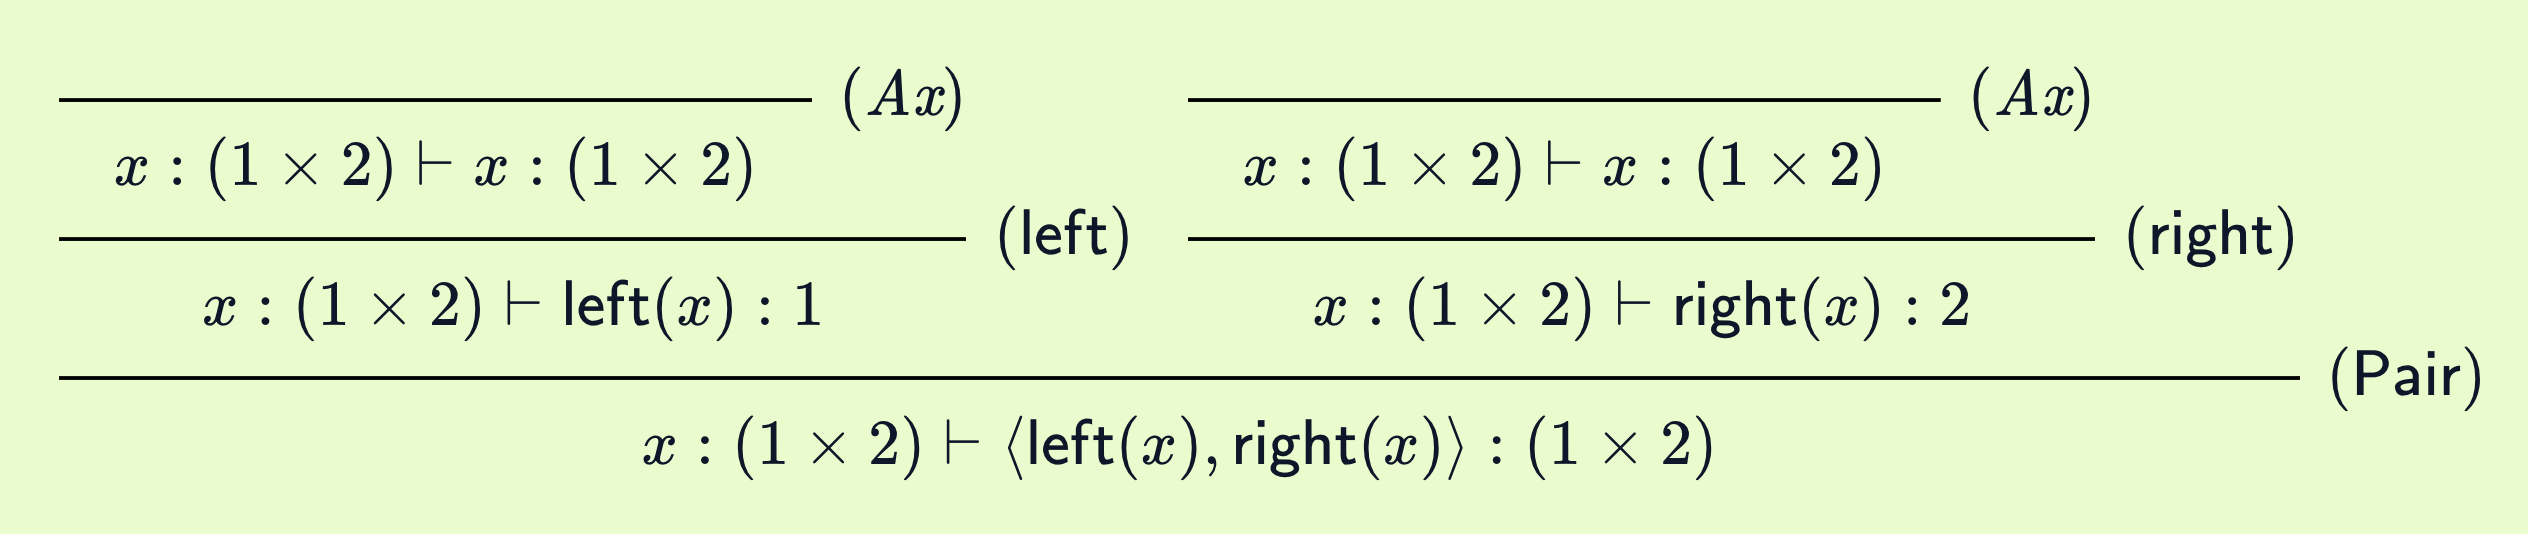
\includegraphics[width=\textwidth]{evaluation/lambda-with-pairs-derivation.png}
    \caption{Derivation in the $\lambda$-calculus with pairs in \projectname{}}
    \label{fig:evaluation:lambda-with-pairs-derivation}
\end{figure}

\subsection{\texorpdfstring{\lbm{}}{Lambda bar mu}}
The calculus \lbm{} was first presented by Curien and Herbelin in 2000 \cite{curien-herbelin:2000}.
\begin{definition}[Syntactic categories in \lbm{}]
    \lbm{} defines three syntactic categories:
    \begin{align*}
        c &\Coloneqq \langle t | e \rangle &(\textit{commands}) \\
        t &\Coloneqq x \alt (\lambda x. t) \alt (\mu \beta. c) &(\textit{terms}) \\
        e &\Coloneqq \alpha \alt (t \cdot e) \alt (\tilde{\mu}x. c) &(\textit{environments})
    \end{align*}
    where $x$ can be any symbol from an infinite list $x, y, z, \ldots$ of \textit{term variables}, and $\alpha$ and $\beta$ can be any symbol from an infinite list $\alpha, \beta, \gamma, \ldots$ of \textit{environment variables} \cite{van-bakel:2024}.
\end{definition}
\begin{definition}[Judgements in \lbm{}]
    \lbm{} defines three types of \textit{judgements} (or \textit{statements}), each typing a syntactic category:
    \begin{align*}
        \text{Judgement} \Coloneqq{} &c: \Gamma \vdash \Delta &(\textit{commands}) \\
        |\  &\Gamma \vdash t: A \alt \Delta &(\textit{terms}) \\
        |\  &\Gamma \alt e: A \vdash \Delta &(\textit{environments})
    \end{align*}
    where $A$ represents a Curry type, $\Gamma$ represents a set of assignments from variables to types, and $\Delta$ represents a set of assignments from co-variables to types.
\end{definition}
\begin{definition}[Type assignment rules in \lbm{}]
    The type assignment rules are defined as follows:
    {
        \derivationfont
        \[
            (\textsf{Cut}): \frac{\Gamma \vdash t: A \alt \Delta \quad \Gamma \alt e: A \vdash \Delta}{\langle t|e \rangle: \Gamma \vdash \Delta}
        \]
    }%
    \vspace{-26pt}
    \begin{center}
        \derivationfont
        \begin{minipage}{.4\textwidth}
            \begingroup
            \addtolength{\jot}{1em}
            \begin{align*}
                (Ax_R)&: \frac{}{\Gamma, x: A \vdash x: A \alt \Delta} \\
                (\arr R)&: \frac{\Gamma, x: A \vdash t: B \alt \Delta}{\Gamma \vdash (\lambda x. t): (A \to B) \alt \Delta} \\
                (\mu)&: \frac{c: \Gamma \vdash \alpha: A, \Delta}{\Gamma \vdash (\mu \alpha. c): A \alt \Delta}
            \end{align*}
            \endgroup
        \end{minipage}%
        \begin{minipage}{.4\textwidth}
            \begingroup
            \addtolength{\jot}{1em}
            \begin{align*}
                (Ax_L)&: \frac{}{\Gamma \alt \alpha: A \vdash \alpha: A, \Delta} \\
                (\arr L)&: \frac{\Gamma \vdash t: A \alt \Delta \quad \Gamma \alt e: B \vdash \Delta}{\Gamma \alt (t \cdot e): (A \to B) \vdash \Delta} \\
                (\tilde{\mu})&: \frac{c: \Gamma, x: A \vdash \Delta}{\Gamma \alt (\tilde{\mu}x. c): A \vdash \Delta}
            \end{align*}
            \endgroup
        \end{minipage}
    \end{center}
\end{definition}
Since vertical bars | in syntax definitions are used to separate alternatives, the vertical bars in the judgements and commands are input using the \LaTeX{} command ``\lstinline{\vert}'' instead. This is not an elegant solution, since ``\lstinline{\vert}'' and the character ``|'' are synonyms of each other, yet they are treated differently and not unified (see \Cref{syntax:normalise} on normalising symbol aliases).

An alternative solution is to not use the character ``|'' to separate alternatives and offer separate input fields in the user interface for each alternative. Although this makes \projectname{} treat both synonyms equally, the additional input fields may bloat the user interface.

\Cref{fig:evaluation:lambda-bar-mu-definition} shows the definitions of the syntax and inference rules in \projectname{}. \Cref{fig:evaluation:lambda-bar-mu-derivations} shows several derivations in \lbm{} in \projectname{}.

\begin{figure}[!htbp]
    \centering
    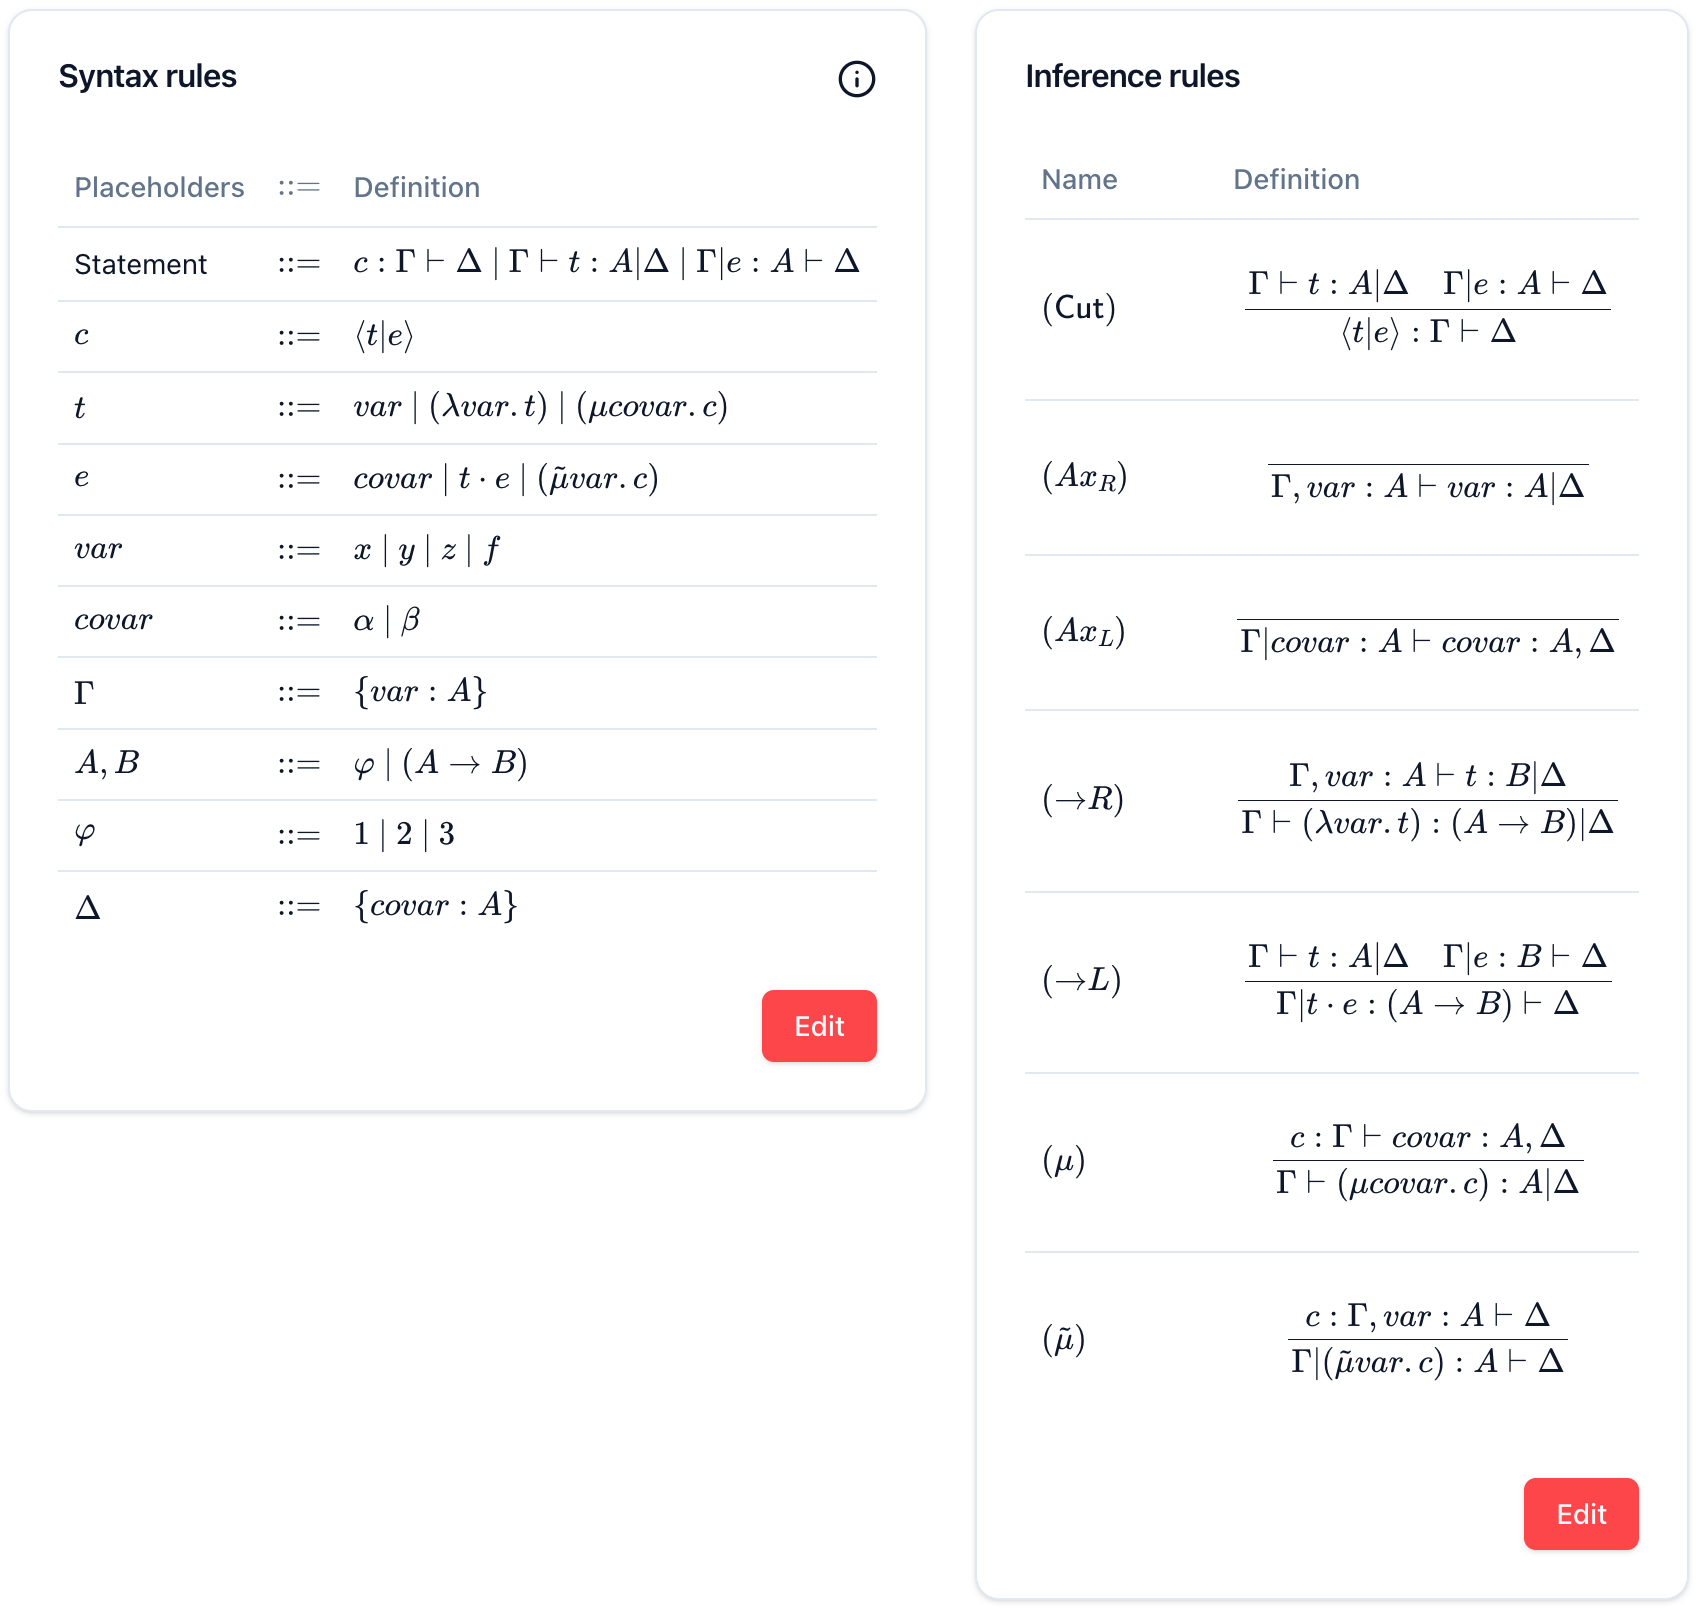
\includegraphics[width=\textwidth]{evaluation/lambda-bar-mu-definition.png}
    \caption{Definition of syntax and inference rules of \lbm{} in \projectname{}}
    \label{fig:evaluation:lambda-bar-mu-definition}
\end{figure}

\begin{figure}[!htbp]
    \centering
    \begin{subfigure}{\textwidth}
        \centering
        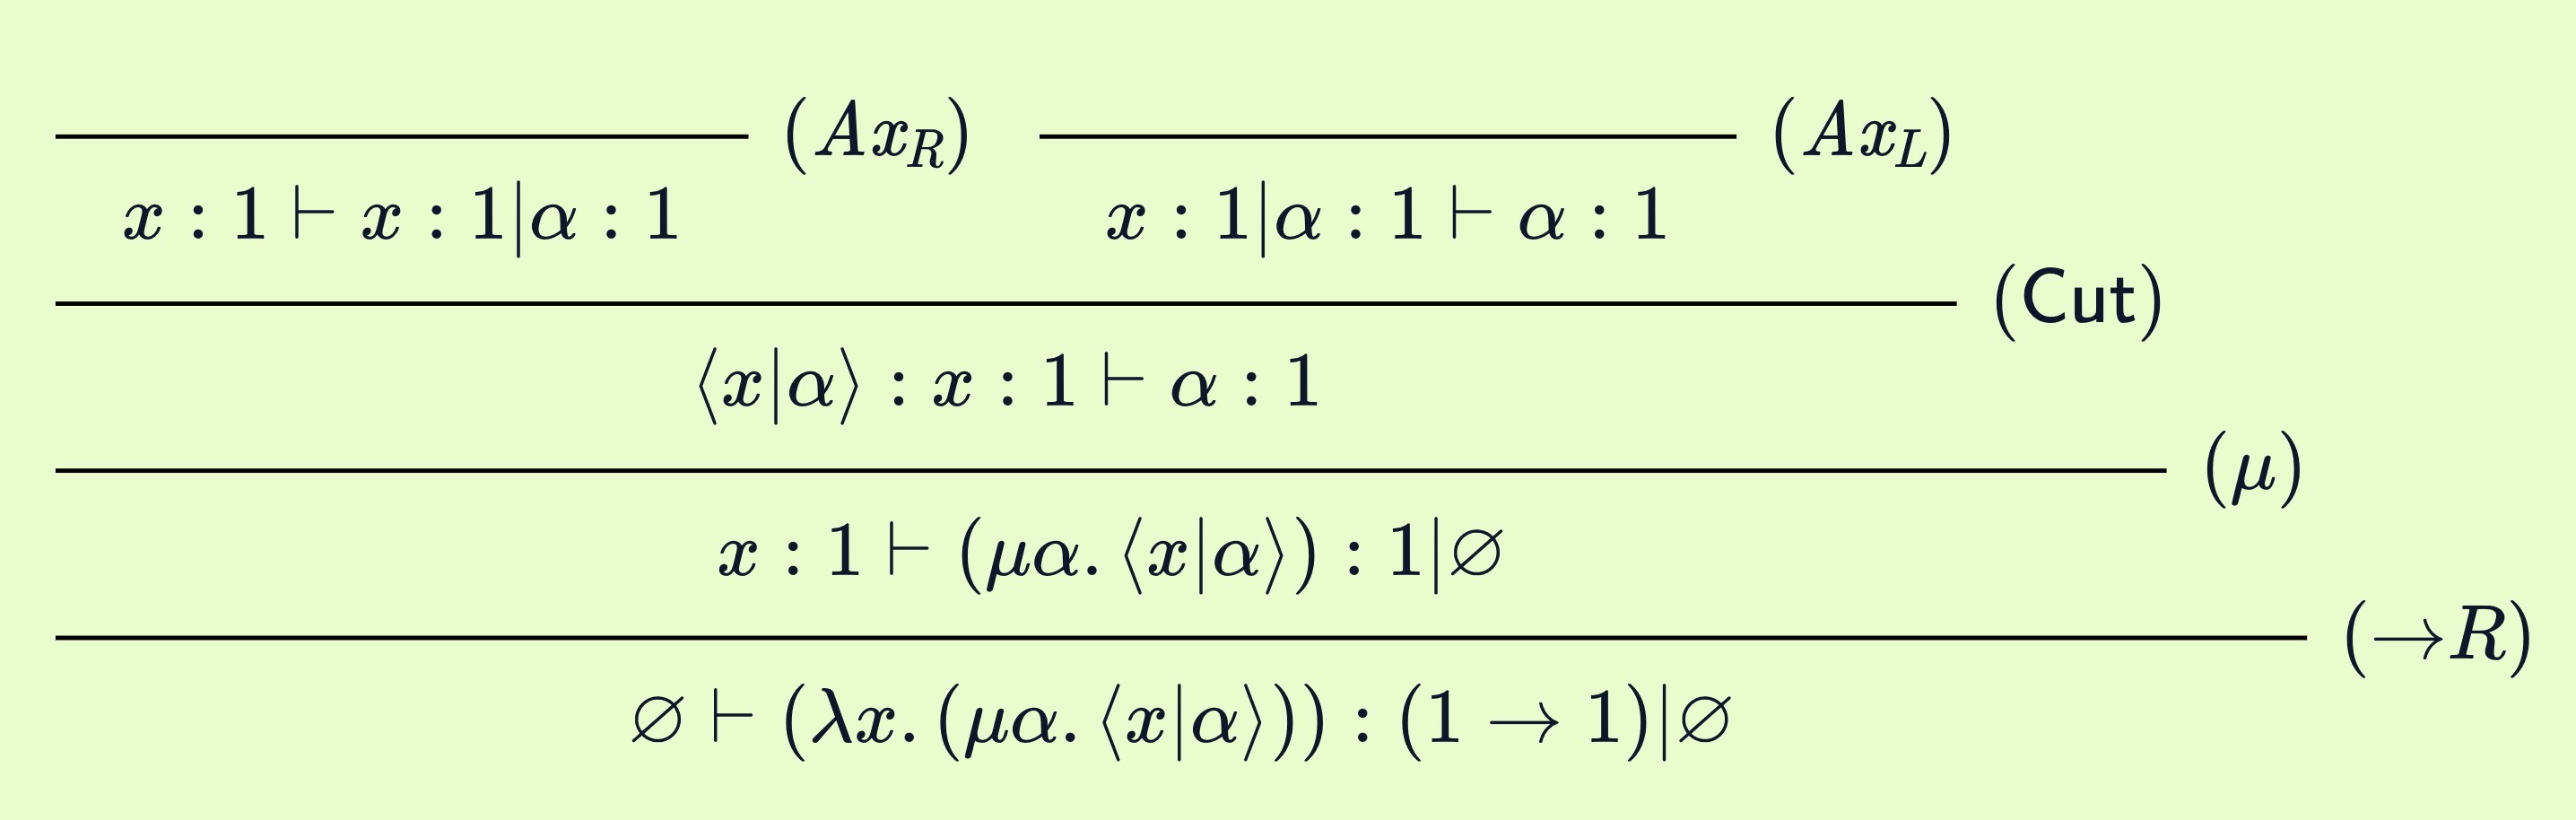
\includegraphics[width=\textwidth]{evaluation/lambda-bar-mu-derivation-mu.png}
        \caption{Derivation using the rule ($\mu$)}
    \end{subfigure}%
    \bigskip\hrulefill\bigskip
    \begin{subfigure}{\textwidth}
        \centering
        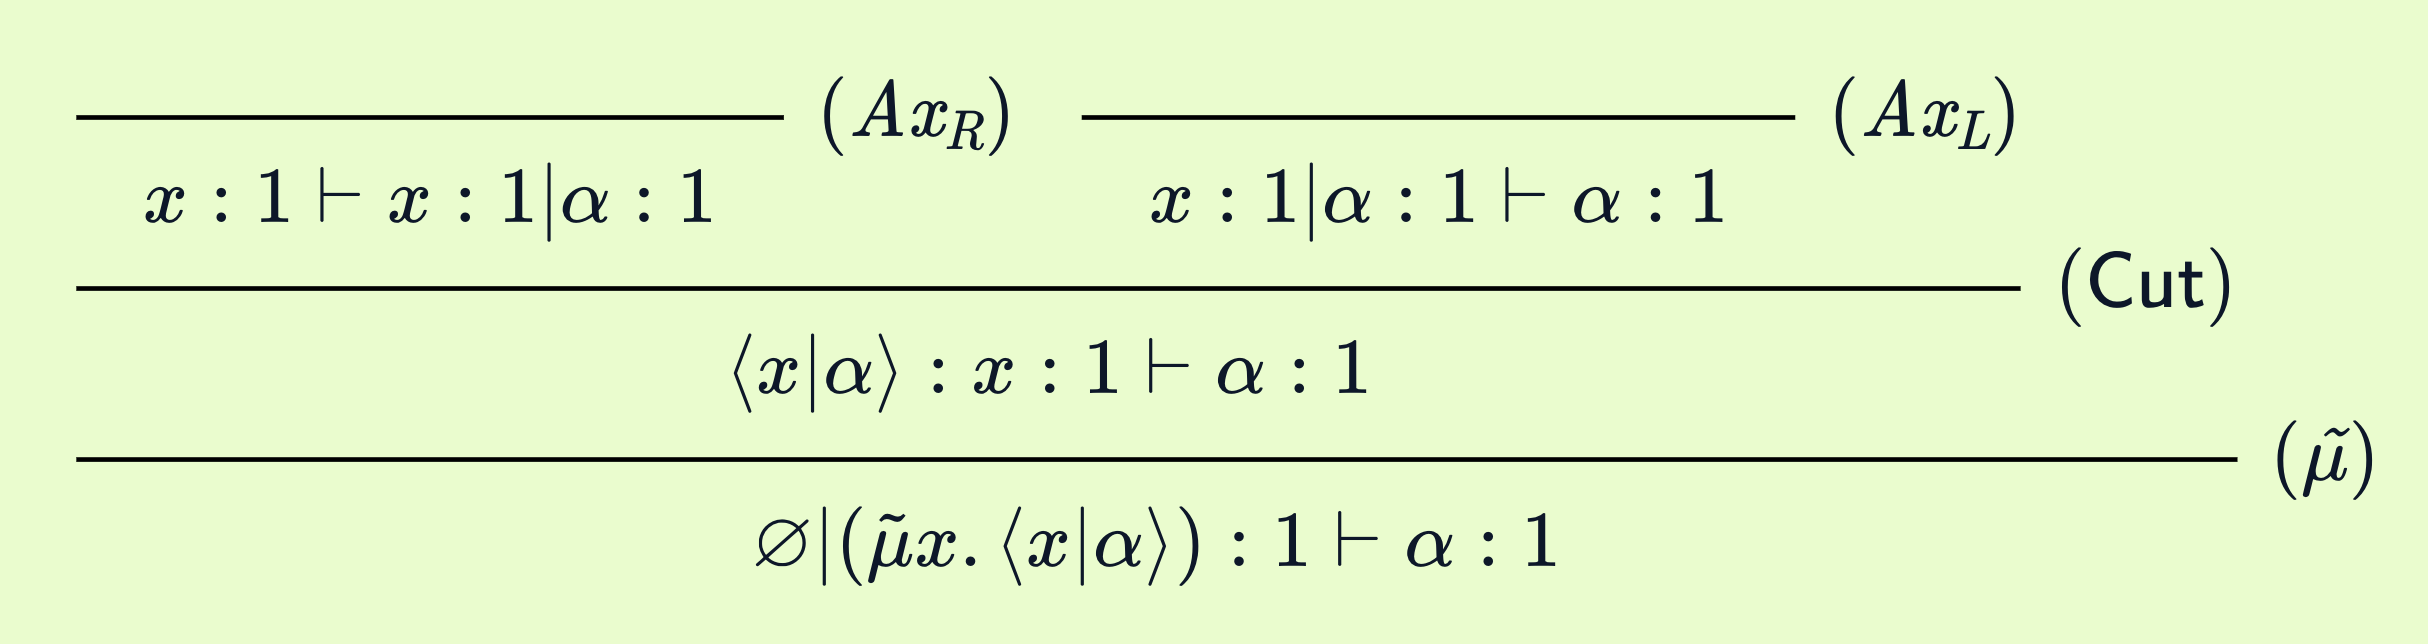
\includegraphics[width=\textwidth]{evaluation/lambda-bar-mu-derivation-tilde-mu.png}
        \caption{Derivation using the rule ($\tilde{\mu}$)}
    \end{subfigure}
    \caption{Derivations in \lbm{} in \projectname{}}
    \label{fig:evaluation:lambda-bar-mu-derivations}
\end{figure}

\section{User experience}
\label{evaluation:ux}
Three students who took the Type Systems module in autumn 2024 were invited to test the web application. User testing was conducted one-on-one over a video call. The users were asked to share their screens so that their interactions with the web application could be observed and analysed.

At the beginning of each session, the users were all told two things: that the web application supported \LaTeX{} input, and that full bracketing was necessary. Afterwards, they were given minimal guidance and navigated the web application mostly on their own, except when they did not know certain \LaTeX{} syntax or had questions about the application.

\subsection{User testing tasks}
The users were asked to complete three tasks: the first task involves deriving a conclusion in the Curry type assignment system for the $\lambda$-calculus, the second task involves extending the $\lambda$-calculus and the Curry type assignment system, and the third task involves deriving a conclusion in the system \textsc{lk}.

\subsubsection{Curry type assignment system for the \lc{}}
In this task, the user is asked to derive the conclusion
\[
    \varnothing \vdash ((\lambda x. x)(\lambda y. y)): (1 \to 1)
\]
in the Curry type assignment system using the web application. This particular conclusion is chosen because it is fairly simple and its derivation requires all three type assignment rules $(Ax)$, $(\arr I)$, and $(\arr E)$.

This task serves as a gentle introduction to the web application. The user only needs to focus on navigating the derivation building part of the web application and not other features, e.g. the syntax and inference rule editors. This task also serves as a quick refresher on building derivation trees, since the user testing was done around half a year after the Type Systems module had ended.

The goal of this task is to evaluate the intuitiveness of the derivation building part of the web application. In particular, the evaluation focuses on how confident the users can input conclusions, rule names, and add premises without guidance, as well as the usefulness of the error messages when the user provides an incorrect derivation.

\subsubsection{\lc{} with pairs}
In this task, the user is asked to extend the syntax of $\lambda$-terms and type assignment rules with pairs, as described in \Cref{evaluation:lambda-pairs}. Afterwards, the user is asked to derive the following conclusion:
\[
    x: (1 \times 2) \vdash \langle \textsf{left}(x), \textsf{right}(x) \rangle: (1 \times 2)
\]
This particular conclusion is chosen because it is fairly simple and its derivation uses all three newly added type assignment rules.

The goal of this task is to evaluate the intuitiveness of the syntax and inference rule editors. In particular, the evaluation focuses on how the users interact with the user interface to check the correctness of their definitions and the usefulness of the error messages and warnings.

\subsubsection{Sequent Calculus \textsc{lk}}
In this task, the user is asked to derive the following conclusion in the system \textsc{lk}:
\[
    ((x \lor y) \to z) \vdash (x \to z)
\]
This particular conclusion is chosen because its derivation requires the rule
\[
    (\arr L): \frac{\Gamma \vdash A, \Delta \quad \Sigma, B \vdash \Pi}{\Gamma, \Sigma, (A \rightarrow B) \vdash \Delta, \Pi}
\]
which may appear quite complicated to users unfamiliar with the system \textsc{lk}, as they would need to pattern match numerous metavariables.

The goal of this task is to evaluate the usefulness of the error messages in the derivation tree and the rule viewers in guiding the users to build a correct derivation in an unfamiliar proof system.

\subsection{User testing findings}
\subsubsection{Redundant parentheses around rule names}
One user asked whether parentheses were needed around the rule names, since there was no indication from the rule name inputs and parenthesised rule names are normally expected in handwritten derivations. The user only realised parentheses were not necessary after he typed the rule name with parentheses, clicked away from the input, and saw the \LaTeX{} display added an extra set of parentheses, as in \Cref{fig:evaluation:rule-name}.

% https://tex.stackexchange.com/questions/218378/forcing-subfigures-to-have-same-height-and-take-overall-x-of-linewidth-in-latex
\begin{figure}[!htbp]
    \sbox\twosubbox{%
    \resizebox{\dimexpr\textwidth-1em}{!}{%
        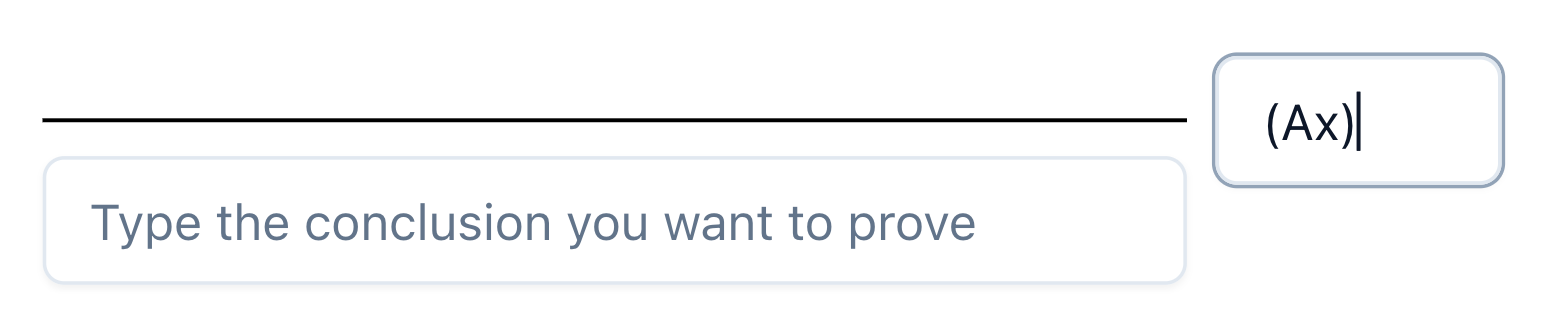
\includegraphics[height=3cm]{evaluation/rule-name-input.png}%
        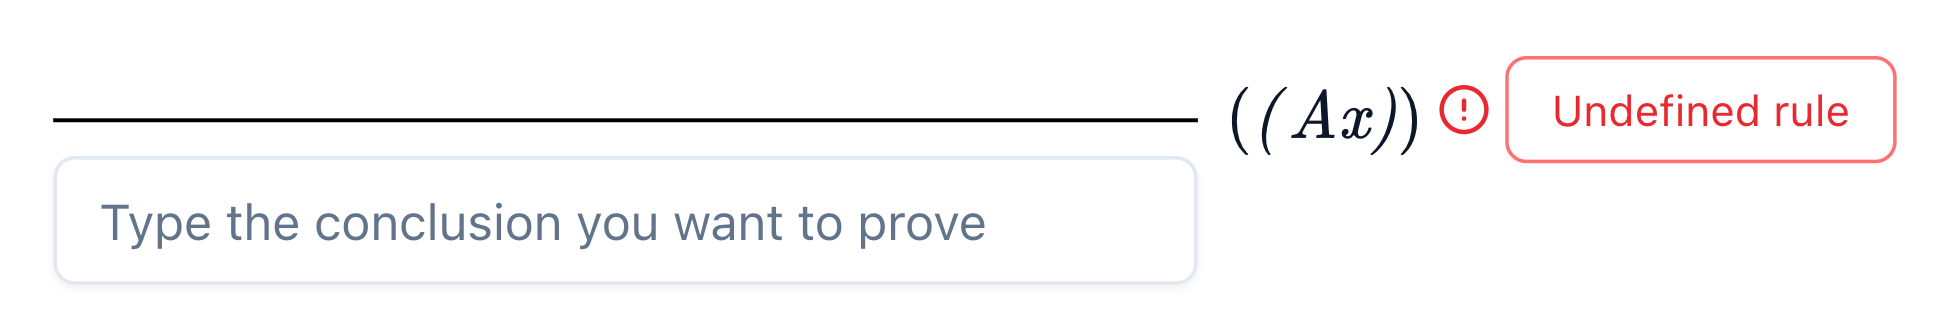
\includegraphics[height=3cm]{evaluation/rule-name-latex.png}%
    }%
    }
    \setlength{\twosubht}{\ht\twosubbox}

    \centering

    \subcaptionbox{There are no parentheses around the rule name input.}{%
        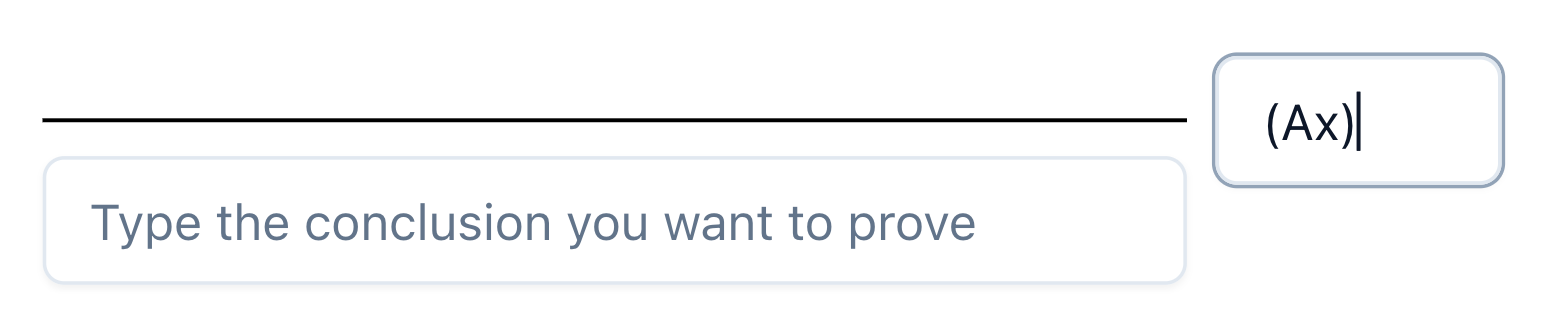
\includegraphics[height=\twosubht]{evaluation/rule-name-input.png}%
    }\quad
    \subcaptionbox{The \LaTeX{} display adds parentheses around the rule name. Note the generic ``undefined rule'' error provided.}{%
        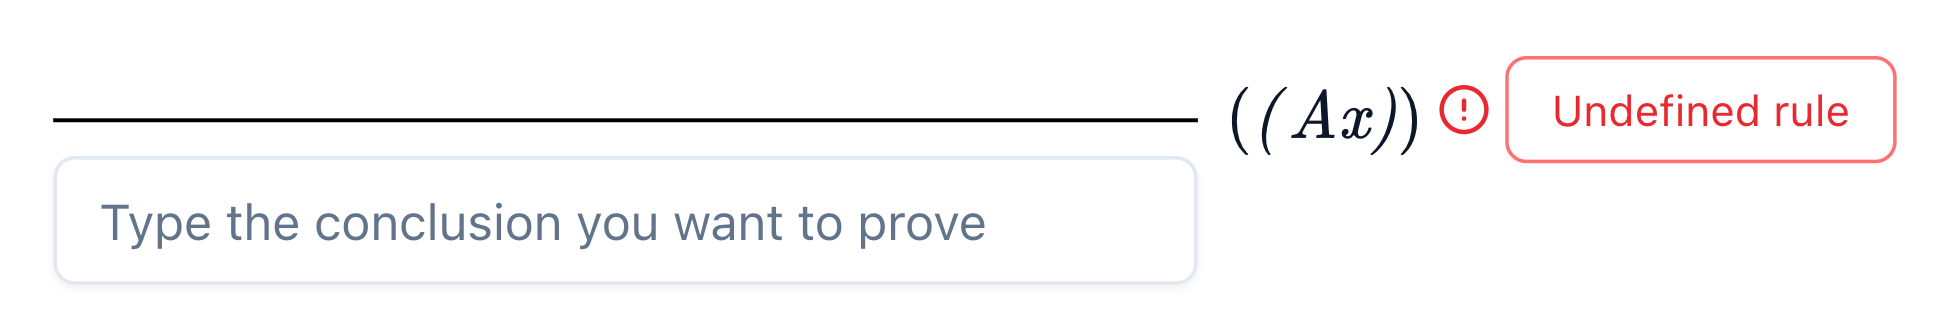
\includegraphics[height=\twosubht]{evaluation/rule-name-latex.png}%
    }
    \caption{It was unclear whether parentheses were needed around the rule name}
    \label{fig:evaluation:rule-name}
\end{figure}

The solution is to both add an entry to the syntax guide and to display a specific error message when superfluous parentheses were added around the rule name input.

\subsubsection{Redundant parentheses around multiset terms}
All users asked whether parentheses were needed around multisets and individual multiset elements, such as $x:1, y:2$ versus $(x:1), (y:2)$ and $(x:1, y:2)$. The question may be common because in the Type Systems module and logic modules in the previous years, students were taught the bracketing conventions and operator associativity of $\lambda$-terms, Curry types, and logical connectives, but never explicitly the bracketing conventions of multisets, which were only introduced in the Type Systems module. Indeed, there was no need to formally introduce bracketing conventions for multisets in the Type Systems module since all derivations were handwritten and there was never any ambiguity when writing multisets in any of the proof systems introduced in the module.

\subsubsection{Unclear indication of correct derivations for colour-blind users}
One user with red-green colour blindness said it took multiple attempts to confirm whether his derivation was correct because the change in background colour from white to pale green appeared quite subtle to him. A comparison between the pale green background colour and a simulated version of what a green-blind user sees is shown in \Cref{fig:evaluation:colour-blind}.

\begin{figure}[!htbp]
    \centering
    \begin{subfigure}{.48\textwidth}
        \centering
        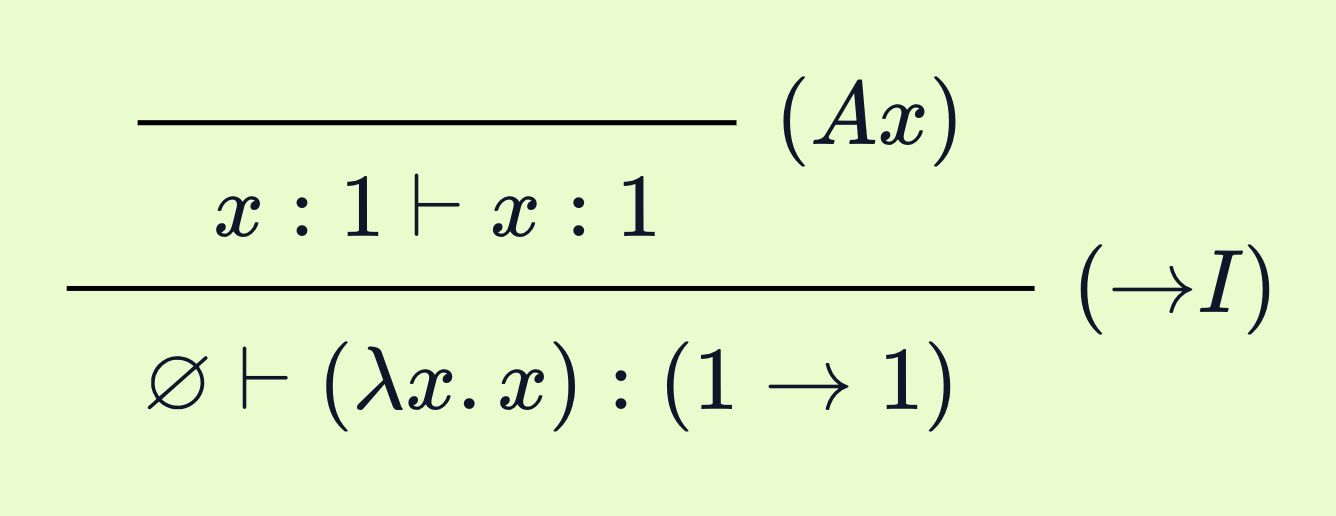
\includegraphics[width=\textwidth]{evaluation/background-normal.png}
        \caption{Pale green background colour}
    \end{subfigure}%
    \quad
    \begin{subfigure}{.48\textwidth}
        \centering
        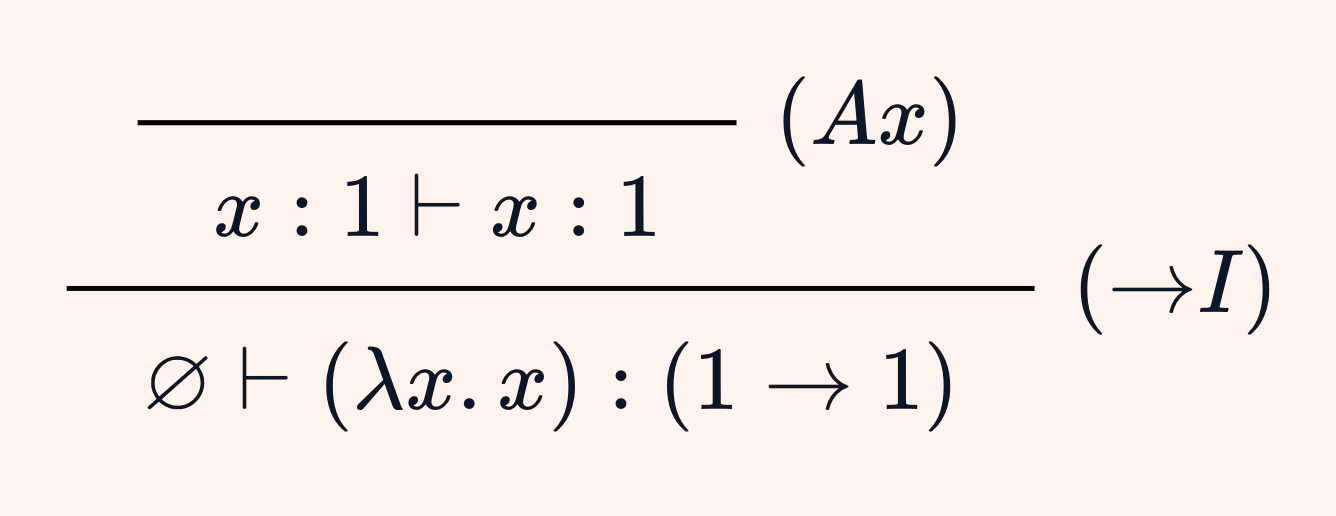
\includegraphics[width=\textwidth]{evaluation/background-colour-blind.jpg}
        \caption{Simulated view of a green-blind user}
    \end{subfigure}
    \caption{What a green-blind person sees when the background colour changes to pale green}
    \label{fig:evaluation:colour-blind}
\end{figure}

The solution is to display additional visual cues, such as a toast, that alert the user when their derivation is correct.

\subsubsection{Mistakenly typing a statement into a rule name input}
Two users mistakenly typed the conclusion of the second premise of a rule into the input for the rule of the first premise, as illustrated in \Cref{fig:evaluation:wrong-premise-input}.

\begin{figure}[!htbp]
    \centering
    \begin{subfigure}{\textwidth}
        \centering
        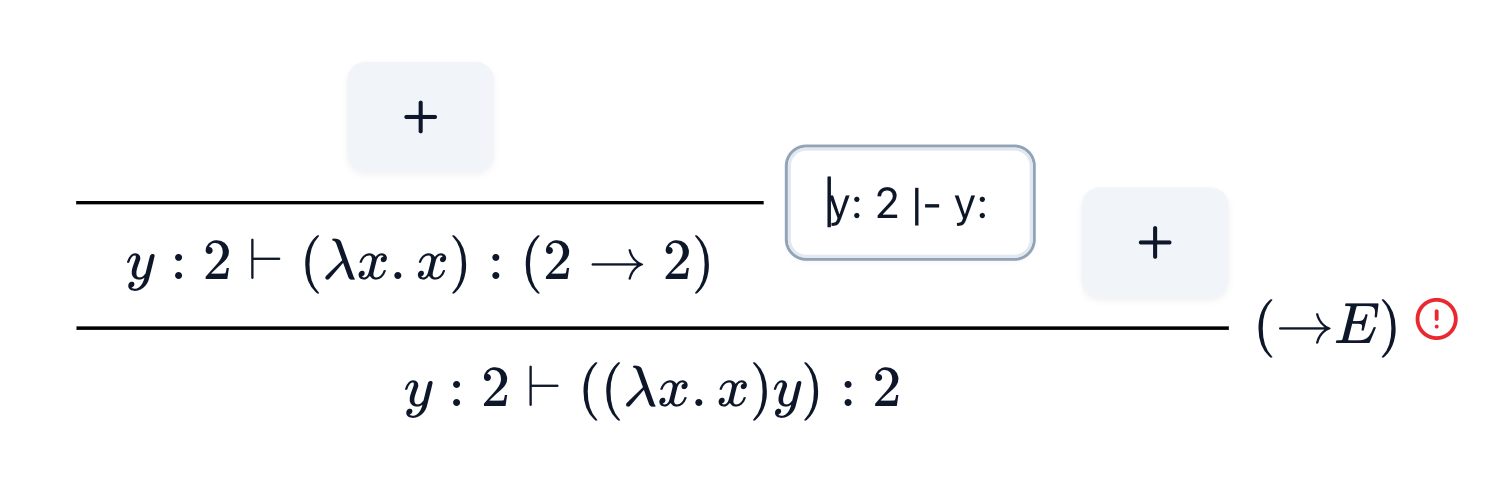
\includegraphics[height=2.5cm]{evaluation/premise-input-wrong.png}
        \caption{The user typed the conclusion instead of the rule name.}
    \end{subfigure}%
    \newline
    \begin{subfigure}{\textwidth}
        \centering
        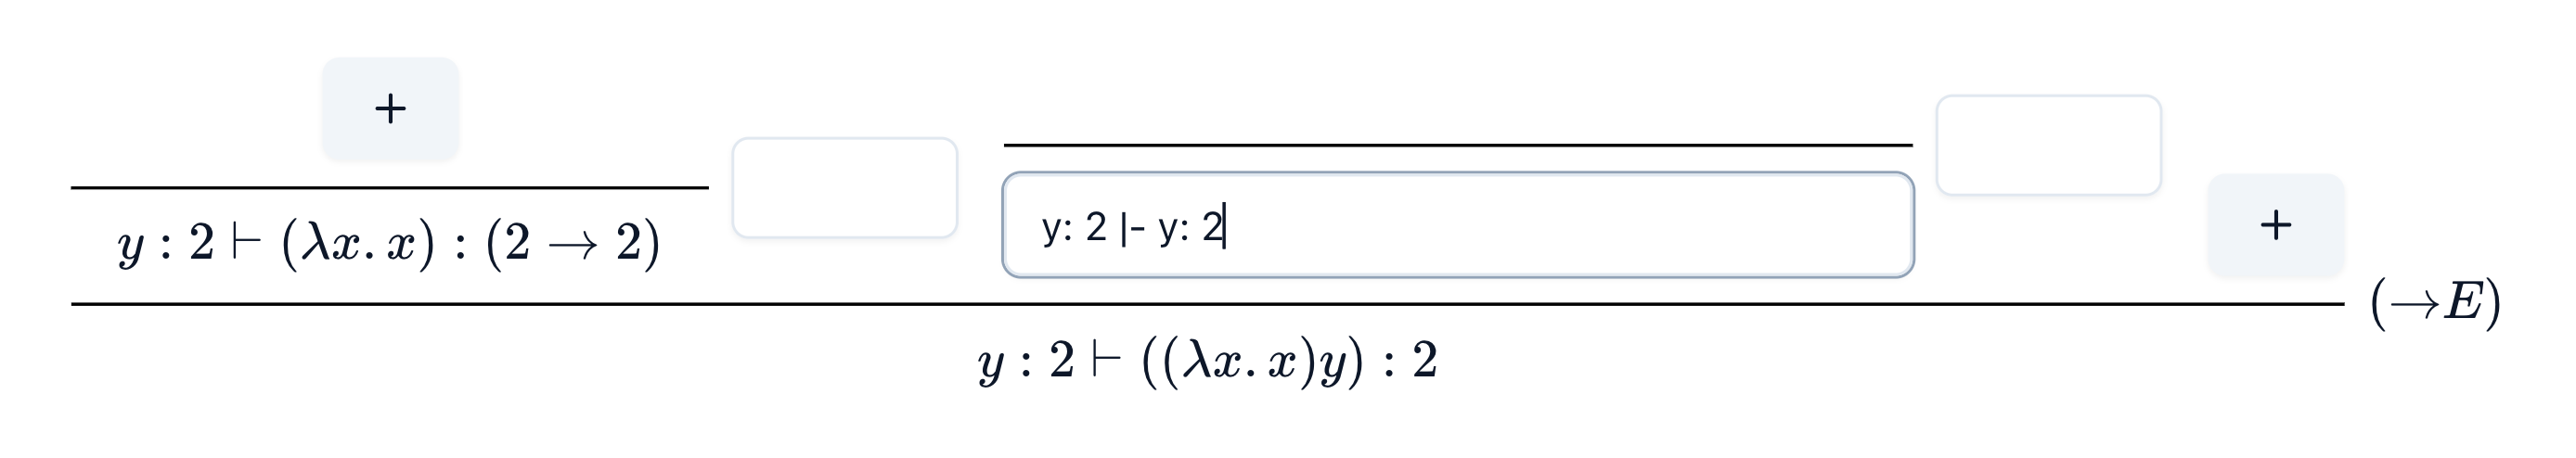
\includegraphics[height=2.5cm]{evaluation/premise-input-correct.png}
        \caption{The user should have added a new premise before typing the conclusion.}
    \end{subfigure}
    \caption{Two users mistakenly typed the conclusion of the second premise of a rule into the input for the rule of the first premise}
    \label{fig:evaluation:wrong-premise-input}
\end{figure}

At the time of testing, there were only placeholders for the conclusion and rule name inputs at the root of the tree: the expectation was that once users input the first conclusion and rule name, they should be able to navigate the rest of the derivation tree without additional guidance. However, user testing showed otherwise. The solution was to add placeholders for all inputs in the derivation tree to indicate whether it should be a conclusion or a rule name.

\subsubsection{Displaying parsing errors before rules are specified}
When completing the first user testing task, one user input all conclusions of the tree before inputting the rule names. Since the web application only displayed errors when the user has specified the rule at the time of testing, the user received no feedback on syntactically incorrect inputs when inputting the conclusions and only received multiple error messages once he started typing the rule names.

The solution is to display two types of errors: general errors regardless of whether the user has specified a rule, and additional specific errors when the user has specified a rule. General errors are displayed when the user inputs a syntactically incorrect statement. Specific errors are displayed when the user inputs a syntactically correct statement which is not compatible with the structure of the corresponding abstract statement, such as when a multiset element with a certain structure cannot be found in the user input, or if some names are incompatible.

\subsubsection{Persisting rules and derivations across reloads}
Two users accidentally closed the tab for the web application during the second task, which required extending the syntax and inference rules. When they opened the application again, the rule definitions and derivation tree were reset since data was not persisted across reloads. Although the users could quickly re-input the rules in this case, it may be more frustrating in other cases when the user accidentally closes the page when defining larger and more complicated proof systems.

The solution is to encode the definitions of the syntax and inference rules as query parameters in the URL and use the \lstinline{localStorage} property \cite{localstorage} to persist derivations across reloads. Though it is possible to store the rule definitions in \lstinline{localStorage} as well, the query parameters are already used to relay information about the rule definitions from the landing page to the derivation builder page. Suppose the rule definitions are only persisted in \lstinline{localStorage}. When the user chooses the pre-defined rules for the $\lambda$-calculus on the landing page, the URL query parameters encode this information and are passed to the derivation builder page, which parses the parameters and sets the rule definitions accordingly. If the user changes to those for the Sequent Calculus in the rule editor, then refreshes the page, the rule definitions and the query parameters become out of sync: the query parameters say the user wants to use the rules for the $\lambda$-calculus, yet the persisted rule definitions are actually those of the Sequent Calculus.
\chapter{Conclusion}
We have developed a web-based proof assistant which lets users define syntax and inference rules in \LaTeX{} and verifies derivations built in the web interface against the user-defined rules. To support these functionalities, we have devised algorithms for parsing syntax rules, inference rules, and concrete terms, as well as verifying derivations by matching names to ASTs. \Cref{fig:conclusion:flowchart} summarises the roles of the various algorithms in this project.

\begin{figure}[!htbp]
    \centering
    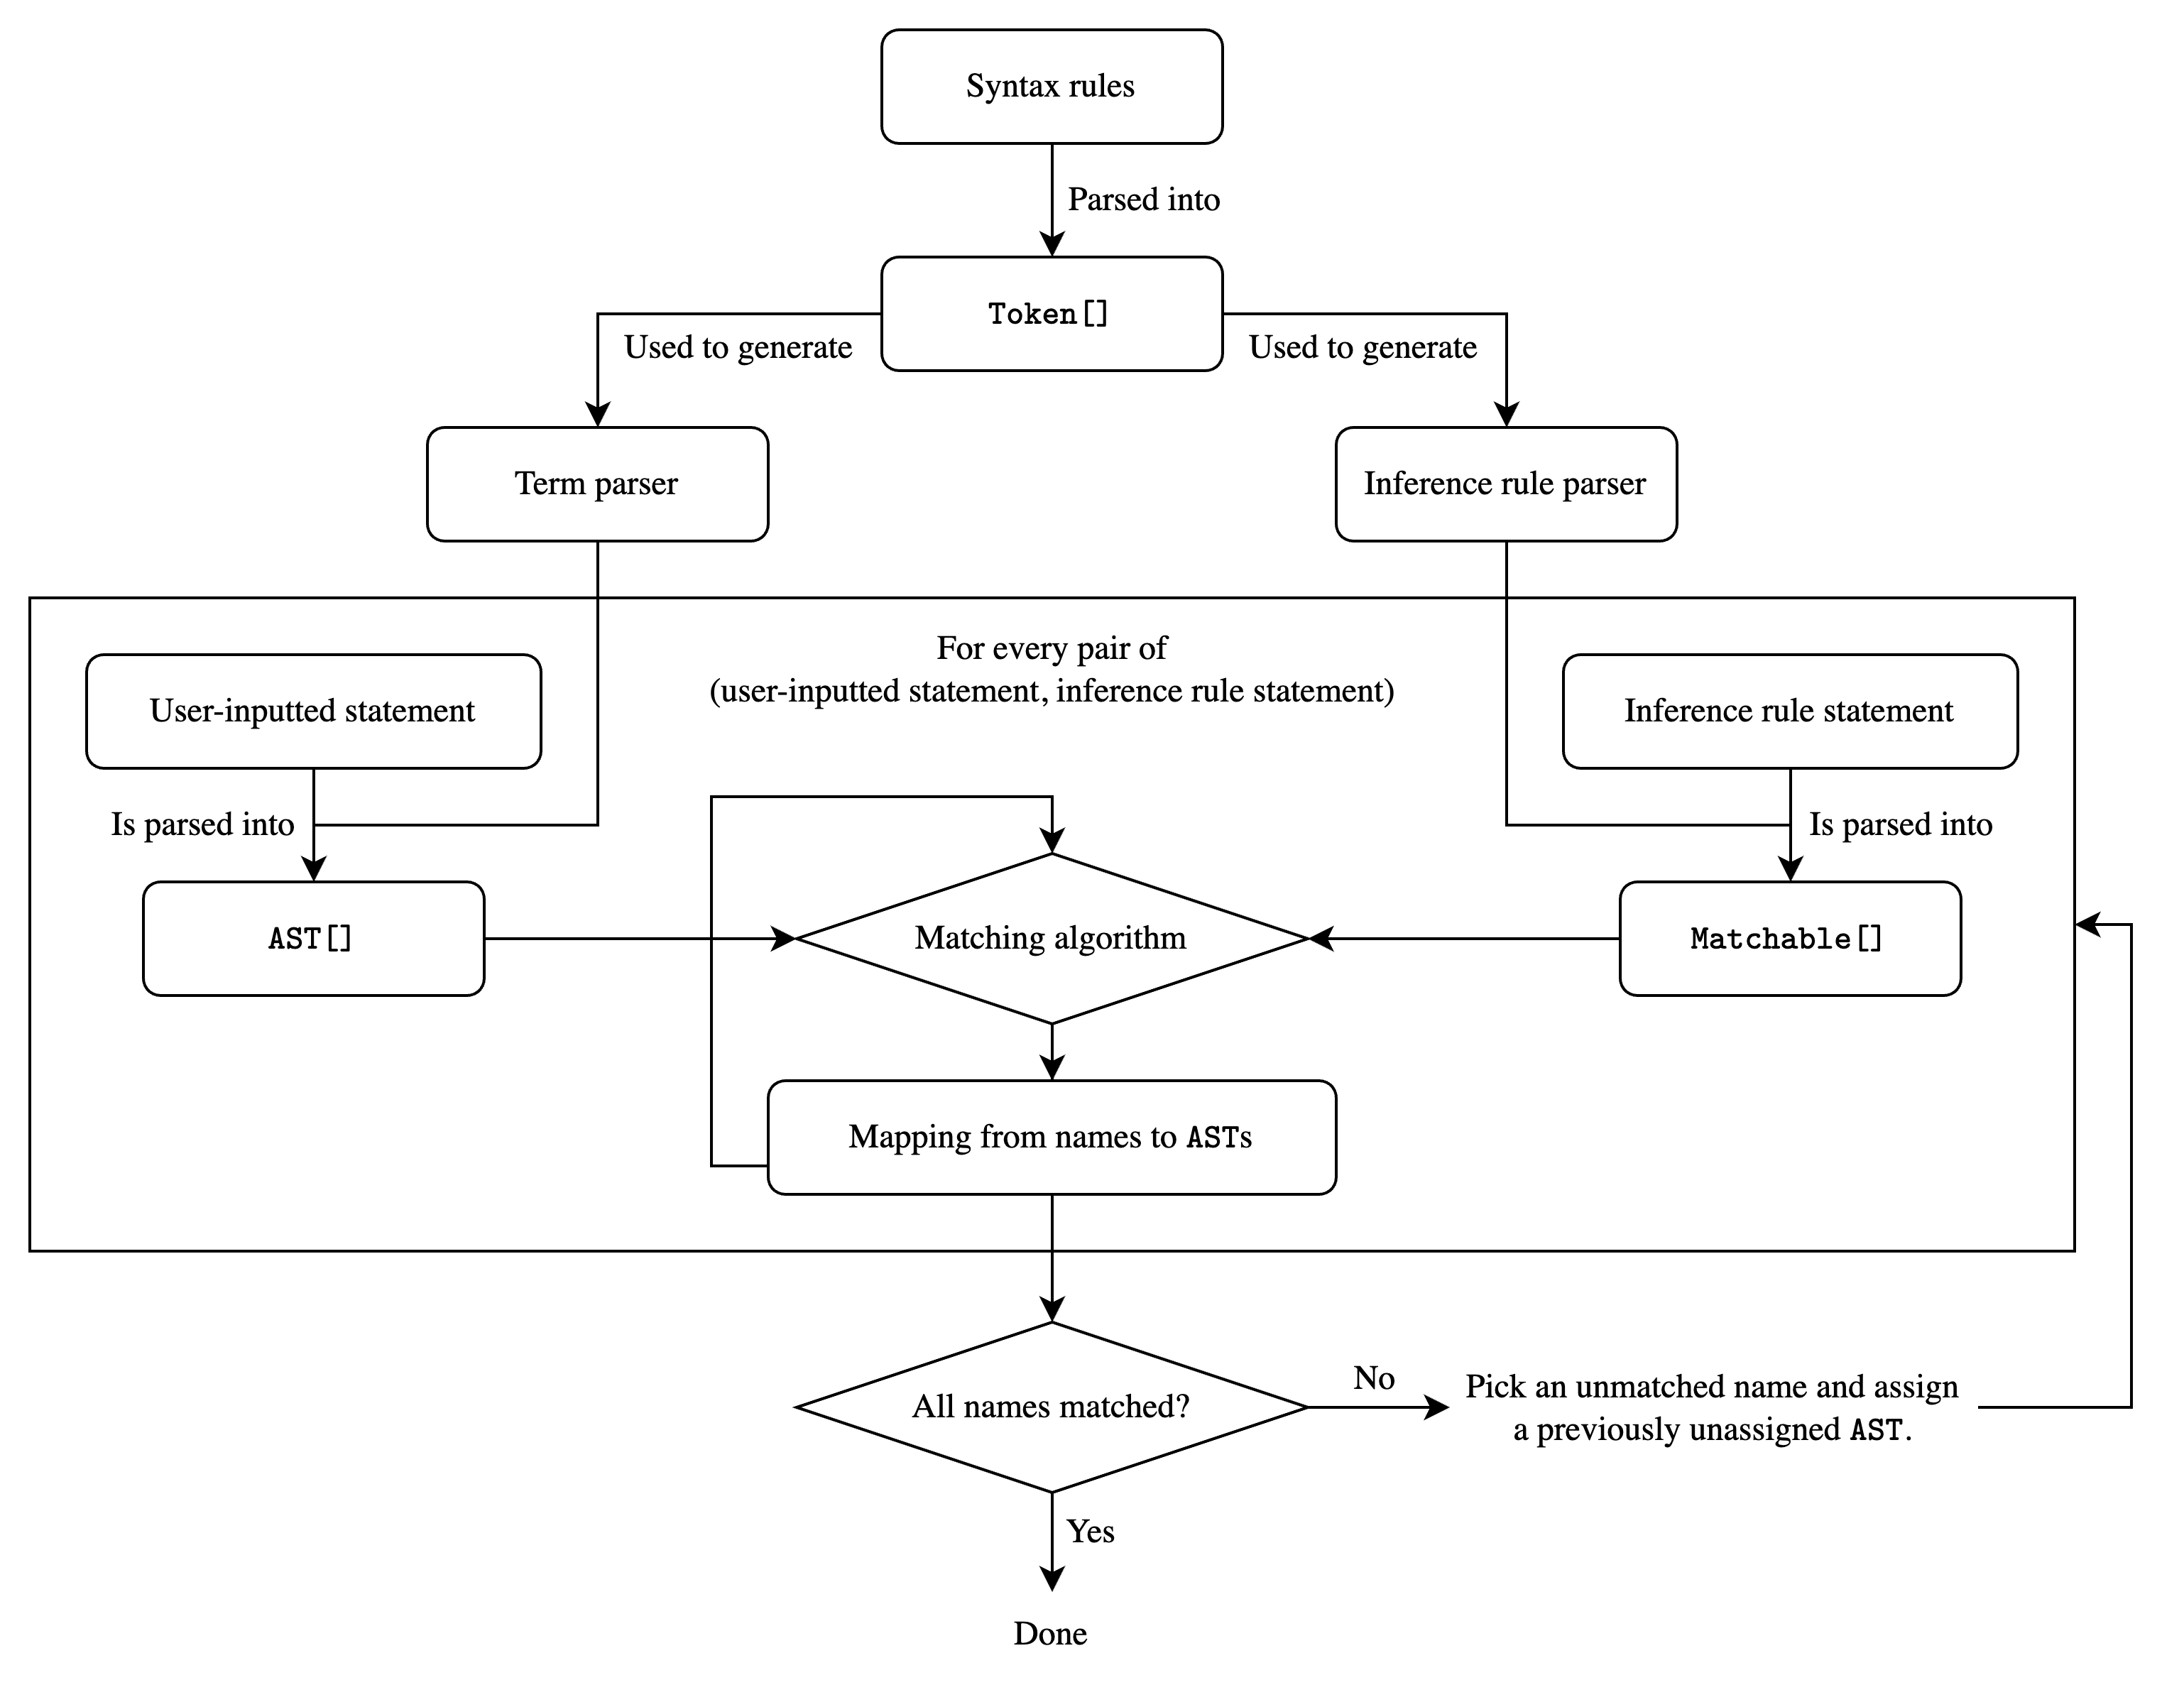
\includegraphics[width=\textwidth]{conclusion/flowchart.png}
    \caption{A flowchart showing the process of verifying whether an inference rule is applied correctly}
    \label{fig:conclusion:flowchart}
\end{figure}

The algorithms were evaluated and refined by testing against example derivations in natural deduction, the simply typed $\lambda$-calculus, the system \textsc{lk}, the $\lambda$-calculus with pairs and product types, and the calculus \lbm. The user experience of the application was evaluated and refined by asking users to build derivations and observing their behaviour.

\section{Future work}
\subsection{Bracketing conventions and abbreviations}
One of the biggest limitations preventing the current web application from becoming a fully ergonomic and intuitive extension of writing derivations by hand is its inability to parse abbreviated terms, including terms that are not fully bracketed.

When writing derivations by hand, we often drop the outermost parentheses and any parentheses that are implied by associativity conventions. For example, the Curry type $(1 \to (2 \to 3))$ is usually abbreviated as $1 \to 2 \to 3$, since $\to$ is right-associative. One solution may be to treat parentheses as special characters and let the user specify operator associativity whenever the definition contains a pair of parentheses. However, it is difficult to determine the operator within the input enclosed by the parentheses. Suppose the user adds symbols to the definition of Curry types:
\[
    A, B \Coloneqq \varphi \alt (A* \to{} +B)
\]
Unless the application treats $\to$ differently from $*$ and $+$, all three symbols are equally likely to be the principal connective in this case. Therefore, the application must either define a set of special symbols as operators or allow the user to specify the operator.

A better solution is to let the user define rewriting rules that capture both associativity and the convention of dropping the outermost parentheses. In the case of Curry types, the user might specify
\begin{align*}
    (A \to (B \to C)) \quad &\to \quad A \to B \to C \\
    (A \to B) \quad &\to \quad A \to B
\end{align*}
where the $\to$ in the middle means ``can be abbreviated as''. One way to preprocess the input according to the re-writing rules is as follows:
\begin{enumerate}
    \item Generate parsers for each of the abbreviations, i.e. the terms on the right of the $\to$.
    \item Apply the abbreviation parsers from top to bottom and stop as soon as a parser succeeds.
    \item Replace the abbreviation with the fully parenthesised form as specified on the left of the $\to$.
    \item Repeat steps 2 to 3 until no more re-writing rules can be applied.
    \item Proceed to the next part of the input.
    \item Repeat steps 2 to 5 until all input is consumed.
\end{enumerate}
Once the input is fully preprocessed, it should be fully parenthesised and ready to be parsed in the manner described in the previous chapters. If the preprocessing algorithm is properly implemented, it should be able to accept both abstract statements and concrete terms as input.

One issue with this solution is that preprocessing from left to right does not always produce the correct result. Consider the abbreviated term $1 \to 2 \to 3 \to 4$. When applied to this term, the preprocessing algorithm described above proceeds as follows:
\begin{enumerate}
    \item Apply the first re-writing rule to get $(1 \to (2 \to 3)) \to 4$.
    \item Apply the second re-writing rule to get $((1 \to (2 \to 3)) \to 4)$.
    \item Neither of the re-writing rules can be applied, so the algorithm terminates.
\end{enumerate}
However, the output should have been $(1 \to (2 \to (3 \to 4)))$ instead. The preprocessing algorithm would have obtained the correct output if it were applied from right to left, since the first step of the algorithm would have returned $1 \to (2 \to (3 \to 4))$.

One way around this issue is to define a special symbol $\cdots$ meaning ``and so on''. The re-writing rules above can be simplified as the rule
\[
    (A_1 \to (A_2 \to \cdots (A_{n-1} \to A_n))) \quad \to \quad A_1 \to A_2 \to \cdots \to A_n
\]
But then the main difficulty becomes interpreting $\cdots$ correctly. Another way around this issue is to enumerate the re-writing rules up to a certain point and not handling any abbreviations beyond that point. For example, the user may choose to only handle abbreviations for Curry types with up to four arrows:
\begin{align*}
    (A \to (B \to (C \to (D \to E)))) \quad &\to \quad A \to B \to C \to D \to E \\
    (A \to (B \to (C \to D))) \quad &\to \quad A \to B \to C \to D \\
    (A \to (B \to C)) \quad &\to \quad A \to B \to C \\
    (A \to B) \quad &\to \quad A \to B
\end{align*}
The latter workaround also works for abbreviations of abstractions in the $\lambda$-calculus, too. In general, the abstraction $(\lambda x_1. (\lambda x_2. \cdots (\lambda x_n. M)))$ can be abbreviated as $\lambda x_1 x_2 \cdots x_n. M$. Ideally, the abbreviation can be expressed by the following re-writing rule:
\[
     (\lambda var_1. (\lambda var_2. \cdots (\lambda var_n. M))) \quad \to \quad \lambda var_1 var_2 \cdots var_n. M
\]
But the same difficulty of interpreting $\cdots$ remains. Instead, enumerating abbreviations up to a certain number of variables would work well:
\begin{align*}
    (\lambda var_1. (\lambda var_2. (\lambda var_3. (\lambda var_4. (\lambda var_5. M))))) \quad &\to \quad \lambda var_1\ var_2\ var_3\ var_4\ var_5. M \\
    &\vdotswithin{\to} \\
    (\lambda var_1. M) \quad &\to \quad \lambda var_1. M
\end{align*}

\subsection{Using and proving lemmas}
Suppose a user wants to prove the following conclusion in the system \textsc{lk}:
\begin{equation}
    \varnothing \vdash (((x \to y) \to x) \to x) \land (((y \to z) \to y) \to y)
    \label{eqn:conclusion:peirce}
\end{equation}
The user can build the derivation as follows:
\[
    \Inf[\land R]{
        \textcolor{ForestGreen}{\Inf[\arr R]{
            \Inf[CR]{
                \Inf[\arr L]{
                    \Inf[\arr R]{
                        \Inf[Ax]{x \vdash y, x}
                    }{\varnothing \vdash (x \to y), x}
                    \quad
                    \Inf[Ax]{x \vdash x}
                }{(x \to y) \to x \vdash x, x}
            }{(x \to y) \to x \vdash x}
        }{\varnothing \vdash ((x \to y) \to x) \to x}}
        \quad
        \textcolor{blue}{\Inf[\arr R]{
            \Inf[CR]{
                \Inf[\arr L]{
                    \Inf[\arr R]{
                        \Inf[Ax]{y \vdash z, y}
                    }{\varnothing \vdash (y \to z), y}
                    \quad
                    \Inf[Ax]{y \vdash y}
                }{(y \to z) \to y \vdash y, y}
            }{(y \to z) \to y \vdash y}
        }{\varnothing \vdash ((y \to z) \to y) \to y}}
    }{\varnothing \vdash (((x \to y) \to x) \to x) \land (((y \to z) \to y) \to y)}
\]
Notice the \textcolor{ForestGreen}{green} and \textcolor{blue}{blue} sub-derivations are identical modulo renaming. It would be convenient to be able to turn the sub-derivation into a lemma, prove the lemma, and be able to use the lemma in another derivation. In this example, the lemma
{
    \derivationfont
    \[
        (\textsf{Peirce}): \frac{}{\varnothing \vdash ((var_1 \to var_2) \to var_1) \to var_1}
    \]
}%
would be proven as follows:
\[
    \Inf[CR]{
        \Inf[\arr L]{
            \Inf[\arr R]{
                \Inf[Ax]{var_1 \vdash var_2, var_1}
            }{\varnothing \vdash (var_1 \to var_2), var_1}
            \quad
            \Inf[Ax]{var_1 \vdash var_1}
        }{(var_1 \to var_2) \to var_1 \vdash var_1, var_1}
    }{(var_1 \to var_2) \to var_1 \vdash var_1}
\]
The derivation for \ref{eqn:conclusion:peirce} could be simplified to
\[
    \Inf[\land R]{
        {\Inf[\textsf{Peirce}]{\varnothing \vdash ((x \to y) \to x) \to x}}
        \quad
        \Inf[\textsf{Peirce}]{\varnothing \vdash ((y \to z) \to y) \to y}
    }{\varnothing \vdash (((x \to y) \to x) \to x) \land (((y \to z) \to y) \to y)}
\]
Most of the work needed to support the use of lemmas is in extending the user interface. It would need to track lemmas and their proofs, since it currently only supports one derivation at a time. The algorithms and data structures can handle most backend tasks associated with the use of lemmas, since a lemma is essentially an inference rule associated with a proof, and the algorithms can handle both custom inference rules and verifying proofs. The only task left is to link the lemma with its proof, which can be done in one of two ways:
\begin{itemize}
    \item Construct the proof using abstract statements and metavariables (e.g. $var_1$ and $var_2$ instead of $x$ and $y$). Since metavariables are forbidden in concrete terms, a new parser is needed for parsing concrete terms and statements in lemma proofs. One way is to parse metavariables as strings and transform them into \lstinline{TerminalAST}s.
    \item Construct the proof using concrete statements compatible with the structures of the statements in the lemma. For example, the lemma $(\textsf{Peirce})$ above may be proved by deriving the conclusion $\varnothing \vdash ((x \to y) \to x) \to x$ instead of $\varnothing \vdash ((var_1 \to var_2) \to var_1) \to var_1$. Matching concrete statements with the structure of a lemma requires more stringent checks than matching concrete statements with the structure of an inference rule when verifying proofs. For example, deriving the conclusion $\varnothing \vdash x \lor (\lnot x)$ does not prove the lemma
    \[
        (\textsf{LEM?}): \frac{}{\varnothing \vdash A \lor B}
    \]
    even though the conclusion is considered compatible with the structure of the conclusion when verifying proofs, since $A$ maps to $x$ and $B$ maps to $(\lnot x)$.
\end{itemize}
% A necessary additional check is to ensure distinct metavariables correspond to distinct concrete terms.
% \appendix
\chapter{First Appendix}

% Handle Dutch surnames with "van", see https://tex.stackexchange.com/questions/40747/bibtex-handling-of-the-dutch-van-name-prefix-with-natbib/40750#40750
\DeclareRobustCommand{\VAN}[3]{#3}
\printbibliography[heading=bibintoc, title={Bibliography}]

\pagebreak
\chapter{Declarations}
\section{Use of generative AI}
I acknowledge the use of ChatGPT 4.0 (OpenAI, https://chatgpt.com/) to generate an outline for background study. I confirm that no content generated by AI has been presented as my own work.

\section{Ethical considerations}
There are no ethical issues associated with this project.

\section{Sustainability}

\section{Availability of data and materials}
The source code is available as a public repository via \url{https://github.com/justinkeung1018/building-derivations}. The web application is currently available via \url{building-derivations.vercel.app}, but this may change in the future. The GitHub repository will contain the updated link.

\end{document}